% ============================================================
%  新能源储能调度系统的设计与实现
%  本科毕业设计论文
%  基于项目 new-energy-sys 实际代码与实验产物
% ============================================================
\documentclass[12pt,a4paper]{ctexbook}

% ---------- 页面设置 ----------
\usepackage[top=2.5cm, bottom=2.5cm, left=3cm, right=2.5cm]{geometry}
\usepackage{fancyhdr}
\pagestyle{fancy}
\setlength{\headheight}{14pt}
\fancyhf{}
\fancyhead[L]{\small 新能源储能调度系统的设计与实现}
\fancyhead[R]{\small \leftmark}
\fancyfoot[C]{\thepage}
\renewcommand{\headrulewidth}{0.4pt}

% ---------- 基础宏包 ----------
\usepackage{graphicx}
\usepackage{float}
\usepackage{booktabs}
\usepackage{longtable}
\usepackage{array}
\usepackage{multirow}
\usepackage{caption}
\usepackage{subcaption}
\usepackage{hyperref}
\hypersetup{hidelinks}
\usepackage{enumitem}
\usepackage{amsmath}
\usepackage{amssymb}
\usepackage{algorithm}
\usepackage{algpseudocode}
\usepackage{listings}
\usepackage{xcolor}
\usepackage{tikz}
\usetikzlibrary{shapes, arrows, positioning, fit, backgrounds}

% ---------- 代码高亮 ----------
\lstset{
  basicstyle=\ttfamily\small,
  breaklines=true,
  frame=single,
  numbers=left,
  numberstyle=\tiny,
  commentstyle=\color{gray},
  keywordstyle=\color{blue},
  stringstyle=\color{red},
  language=Python,
  showstringspaces=false,
  tabsize=2,
  captionpos=b
}

% ---------- 引用 ----------
\usepackage[sort&compress]{gbt7714}
\bibliographystyle{gbt7714-numerical}

% ---------- 其他 ----------
\usepackage{titletoc}
\usepackage{appendix}
\setlength{\parskip}{0.5ex plus 0.2ex minus 0.2ex}
\setlength{\parindent}{2em}
\renewcommand{\thefigure}{\thechapter-\arabic{figure}}
\renewcommand{\thetable}{\thechapter-\arabic{table}}
\renewcommand{\theequation}{\thechapter-\arabic{equation}}

% ---------- 文档信息 ----------
\title{新能源储能调度系统的设计与实现}
\author{}
\date{}

\begin{document}

% ============================================================
%  封面（留空，待学校模板替换）
% ============================================================
\begin{titlepage}
\vspace*{6cm}
\begin{center}
{\Huge\bfseries 新能源储能调度系统\\[12pt] 的设计与实现}\\[3cm]
{\large 本科毕业设计论文}\\[4cm]
\begin{tabular}{rl}
\textbf{学\quad 院：} & 信息科学技术学院 \\
\textbf{专\quad 业：} & 计算机科学与技术 \\
\textbf{学\quad 号：} & \rule{3cm}{0.4pt} \\
\textbf{学生姓名：} & \rule{4cm}{0.4pt} \\
\textbf{指导教师：} & \rule{4cm}{0.4pt} \\[2cm]
\end{tabular}
\vfill
{\large 二〇二六年五月}
\end{center}
\end{titlepage}

% ============================================================
%  原创性声明（留空）
% ============================================================
\newpage
\thispagestyle{empty}
\vspace*{4cm}
\begin{center}
{\Large\bfseries 原创性声明及使用授权书}\\[2cm]
\end{center}
{\large 本人郑重声明：所呈交的学位论文，是本人在导师指导下独立完成的成果。……}\\[1cm]
\vfill

\newpage

% ============================================================
%  摘要
% ============================================================
\chapter*{摘要}
\addcontentsline{toc}{chapter}{摘要}

随着全球能源转型的深入，光伏发电在电力系统中的占比持续攀升。然而，光伏出力受天气条件影响呈现显著的间歇性与波动性，给电力系统的安全运行与市场收益带来严峻挑战。储能系统（Battery Energy Storage System, BESS）可通过充放电策略平抑光伏出力波动、利用电价峰谷差进行套利，但如何基于不完美的光伏功率预测制定鲁棒的储能调度策略，是一个兼具理论价值与工程意义的课题。

本文设计并实现了一套完整的新能源储能调度仿真系统，涵盖数据采集与标准化、光伏功率预测、储能优化调度、电池退化分析、真实电站参照仿真和可视化展示六大模块。在光伏预测侧，以LightGBM梯度提升树为主模型（测试集$t+24h$归一化均方根误差nRMSE=0.1225），并系统对比了TCN、CNN-LSTM、Attention-LSTM等深度学习模型的预测性能。在储能调度侧，从固定阈值策略出发，经过策略敏感性分析、24小时前瞻滚动优化调度、储能配置与目标函数权衡分析，逐步演进至电池退化净收益修正和Rawhide Prairie Solar真实电站参数参照仿真。在调度策略智能优化方面，提出了一种两阶段神经网络策略蒸馏方法，以滚动优化调度为首步决策教师，训练神经网络学生模型直接输出充放电离散动作，测试集准确率达0.9908，宏平均F1分数0.9749。此外，系统还实现了基于Vue.js和FastAPI的前后端分离可视化平台，支持模型对比、调度仿真、策略治理和数据探索等功能。

本系统的核心贡献在于构建了一条从数据到决策的完整可复现实验链路，并通过多阶段迭代验证了"传统机器学习预测 + 滚动优化调度 + 神经网络策略蒸馏"技术路线的可行性。系统所有模块均经过严格的质量门禁验证，代码与实验产物可复现。

\vspace{1cm}
\noindent\textbf{关键词：}光伏功率预测；储能调度优化；LightGBM；深度学习；策略蒸馏；电池退化

\newpage

\chapter*{Abstract}
\addcontentsline{toc}{chapter}{Abstract}

As the global energy transition deepens, the share of photovoltaic (PV) generation in power systems continues to rise. However, PV output exhibits significant intermittency and volatility due to weather conditions, posing serious challenges to system security and market revenue. Battery Energy Storage Systems (BESS) can smooth PV output fluctuations and exploit electricity price spreads through charge-discharge strategies. Yet, how to formulate robust storage dispatch strategies based on imperfect PV power forecasts remains a problem of both theoretical value and engineering significance.

This thesis designs and implements a comprehensive new energy storage dispatch simulation system, encompassing six modules: data acquisition and standardization, PV power forecasting, storage dispatch optimization, battery degradation analysis, real-plant reference simulation, and visualization. On the prediction side, LightGBM gradient boosting serves as the primary model (test-set $t+24h$ normalized RMSE = 0.1225), with systematic comparisons against TCN, CNN-LSTM, and Attention-LSTM deep learning models. On the dispatch side, starting from a fixed-threshold strategy, the system progresses through strategy sensitivity analysis, 24-hour look-ahead rolling optimization, configuration-objective trade-off analysis, battery degradation net-value adjustment, and Rawhide Prairie Solar reference simulation using publicly available plant parameters. For intelligent dispatch, a two-stage neural policy distillation method is proposed: using the rolling optimizer as the first-step teacher, a neural student model directly outputs discrete charge-discharge actions, achieving a test accuracy of 0.9908 and a macro F1 score of 0.9749. The system also includes a Vue.js and FastAPI-based visualization platform supporting model comparison, dispatch simulation, strategy governance, and data exploration.

The core contribution of this system is a complete, reproducible experimental chain from data to decision, validated through multi-stage iteration. All modules pass rigorous quality gates, and both code and experimental artifacts are reproducible.

\vspace{1cm}
\noindent\textbf{Keywords:} PV power forecasting; storage dispatch optimization; LightGBM; deep learning; policy distillation; battery degradation

\newpage

% ============================================================
%  目录
% ============================================================
\tableofcontents
\newpage

% ============================================================
%  第一章 绪论
% ============================================================
\chapter{绪论}

\section{选题背景与意义}

在全球碳中和目标的推动下，以光伏为代表的可再生能源发电正经历前所未有的高速增长。根据国际能源署（IEA）的数据，2024年全球光伏新增装机容量突破500 GW，累计装机超过2 TW\cite{iea-pvps-2025}。中国作为全球最大的光伏市场，光伏发电在电力系统中的占比持续攀升，部分省份午间光伏渗透率已超过40\%。\cite{iea-pvps-2025,cn-storage-config-review-2025}

然而，光伏发电的固有特性——间歇性（intermittency）和波动性（volatility）——给电力系统的安全经济运行带来了深刻挑战。光伏出力严格依赖于太阳辐照度、云量、温度等气象条件，在分钟至小时尺度上呈现剧烈波动。当大规模光伏接入电网后，"鸭子曲线"效应愈发显著：午间光伏满发导致净负荷骤降，傍晚光伏退出后净负荷急剧攀升，给常规机组的爬坡能力和系统调峰带来巨大压力\cite{duck-curve-caiso-2016}。

储能系统（Battery Energy Storage System, BESS）被广泛认为是解决上述问题的关键技术手段\cite{bess-review-2023,cn-storage-config-review-2025}。电化学储能具有响应速度快（毫秒级）、功率密度高、模块化部署灵活等优势，可通过充电吸收过剩光伏出力、在电价高峰或负荷高峰时段放电，实现以下多重目标：（1）平抑光伏出力波动，降低系统爬坡压力；（2）利用电价峰谷差进行能量套利（energy arbitrage），提升项目经济收益；（3）提供辅助服务（调频、备用等），增强系统灵活性。已有研究表明，预测误差补偿、波动平抑、容量配置、消纳约束和电压控制往往需要协同考虑，单纯追求某一时段的套利收益容易忽略系统运行约束\cite{xie-hybrid-storage-2021}。

然而，储能的调度决策高度依赖于对未来光伏出力的预测。预测越准确，调度策略越能趋近最优；预测偏差轻则导致套利收益下降，重则引发电量短缺或电池过度循环老化。因此，构建一套从光伏功率预测到储能调度优化的完整技术链路，并系统评估预测不确定性对调度收益的影响，对于推动"光伏+储能"项目的工程落地具有重要的理论与实践意义。\cite{xie-hybrid-storage-2021,milp-dispatch-2021,drl-energy-storage-2023,battery-degradation-review-2021}

本课题旨在设计并实现一套完整的新能源储能调度仿真系统，以美国科罗拉多州真实光伏电站（PVDAQ System 10）和Platte River Power Authority旗下的Rawhide Prairie Solar电站为参照对象，基于公开光伏数据、气象再分析数据、历史天气预报和电价数据，实现从数据采集、功率预测、储能调度到可视化展示的全链路仿真与优化\cite{pvdaq-nrel,rawhide-nrel}。\cite{pvdaq-nrel,nsrdb-nrel,opsd-datapackage-2020,opsd-wiese-2019,open-meteo-2023,rawhide-nrel}

\section{国内外研究现状}

\subsection{光伏功率预测研究现状}

光伏功率预测方法可大致分为物理模型方法、统计机器学习方法和深度学习方法三大类。\cite{pv-physical-model-2019,pv-deep-review-2025}

物理模型方法基于光伏组件的等效电路模型（如单二极管模型、双二极管模型），结合数值天气预报（Numerical Weather Prediction, NWP）提供的辐照度和温度预报，通过求解光伏出力曲线得到功率预测值\cite{pv-physical-model-2019}。该类方法的优势在于不需要大量历史发电数据即可建立模型，但其精度高度依赖于NWP预报的时空分辨率和光伏组件参数的准确标定。

统计机器学习方法以历史发电数据和相关气象特征为输入，通过回归模型学习输入-输出之间的映射关系。常用的算法包括支持向量回归（SVR）、随机森林（Random Forest）、极端梯度提升（XGBoost）和轻量梯度提升机（LightGBM）等\cite{lightgbm-2017}。其中，LightGBM因其训练速度快、内存占用小、对类别特征支持好等特点，在光伏预测竞赛和工业应用中表现出色。国内近年综述也指出，深度学习方法虽然在时序特征提取方面具有优势，但模型效果受到数据规模、天气类型、预测时间尺度和特征可获得性的共同制约\cite{pv-deep-review-2025}。因此，在工程系统中保留LightGBM作为稳定主模型，同时将深度学习模型作为对照实验，是更稳妥的技术路线。\cite{random-forest-2001,xgboost-2016,catboost-2018,lightgbm-2017}

深度学习方法以卷积神经网络（CNN）、循环神经网络（RNN）及其变体长短期记忆网络（LSTM）和门控循环单元（GRU）为代表，近年来在时间序列预测领域取得了显著进展\cite{lstm-pv-2021,tcn-wan-2019}。时序卷积网络（Temporal Convolutional Network, TCN）通过膨胀因果卷积实现长距离时序依赖建模，在多个序列预测基准上超越了LSTM\cite{tcn-wan-2019}。CNN-LSTM混合模型则将CNN的局部模式提取能力与LSTM的时序记忆能力相结合\cite{wang-cnn-lstm-2019}；面向日前小时级预测的Attention-CNN-LSTM研究进一步说明，注意力机制可用于强化多变量输入中的关键时段和关键特征\cite{qu-attention-cnnlstm-2021}。然而，在训练样本有限、特征维度较高、物理约束严格的光伏预测场景下，深度学习方法是否一定能优于梯度提升树模型，仍是一个开放问题。

\subsection{储能调度优化研究现状}

储能调度优化问题的核心是在满足电池物理约束（荷电状态上下限、充放电功率上限、充放电效率、循环寿命等）的前提下，最大化调度收益或最小化运行成本。根据优化方法的不同，可分为基于规则的方法、基于数学规划的方法和基于强化学习的方法。\cite{bess-review-2023,milp-dispatch-2021,drl-energy-storage-2023}

基于规则（Rule-based）的方法采用预设的充放电阈值或分时电价表进行调度决策。例如，当预测光伏出力超过负荷需求且电价低于某阈值时充电，当电价高于某阈值时放电。该类方法的优点是计算简单、可解释性强，缺点是难以适应电价分布和天气条件的变化。\cite{bess-review-2023,milp-dispatch-2021}

基于数学规划的方法将调度问题形式化为线性规划（LP）、混合整数线性规划（MILP）或动态规划（DP）问题\cite{milp-dispatch-2021}。该类方法可在给定预测信息的条件下保证解的全局最优性，但计算复杂度随规划时域和状态空间呈指数增长，难以在实时或小时级滚动场景中保证时效性。日前--日内两阶段滚动优化和模型预测控制（Model Predictive Control, MPC）在源荷储协同调度中被广泛用于缓解预测误差和运行状态变化带来的偏差\cite{bo-two-stage-rolling-2025,li-mpc-microgrid-2025}，这也构成了本文采用24小时前瞻滚动调度的文献基础。

基于深度强化学习（Deep Reinforcement Learning, DRL）的方法将调度问题建模为马尔可夫决策过程（MDP），通过与环境交互学习最优策略\cite{drl-energy-storage-2023}。DQN、DDPG、PPO等算法已被应用于储能调度场景，也有研究将注意力机制引入日前--日内多源储能调度，以提升智能体对预测误差和储能状态的关注能力。DRL方法可在线适应环境变化，但其训练不稳定、策略不可解释等问题仍是工程落地的障碍。近年来，策略蒸馏（Policy Distillation）技术\cite{policy-distillation-2016}被提出用于将复杂的教师策略（如滚动优化结果）压缩为学生神经网络模型，从而在保持策略质量的同时大幅降低在线推理复杂度。

\subsection{电池退化建模研究现状}

锂离子电池在循环使用过程中会经历不可逆的容量衰减（aging/degradation），主要机制包括固体电解质界面膜（SEI）增长、活性材料损失和锂库存消耗\cite{battery-degradation-review-2021}。在储能调度场景中，循环深度和SOC工作区间直接影响电池的健康状态（State of Health, SOH）衰减速率。雨流计数法（Rainflow Counting）是材料疲劳分析中广泛使用的循环计数方法，已被IEC 61400等标准采纳用于电池循环寿命评估，也常用于储能应用中的电池寿命估计\cite{rainflow-soc-2022}。将电池退化成本纳入调度目标函数，可避免将电池推到极端SOC区间，在收益最大化和寿命保护之间取得平衡。

\section{论文主要工作}

本论文完成的主要工作包括以下几个方面：

（1）\textbf{数据地基构建}：从PVDAQ、NSRDB、OPSD和Open-Meteo等多个公开数据源采集光伏发电、气象再分析、电价和天气预报数据，通过统一时间对齐、缺失值处理、异常值检测和特征工程，构建了覆盖2020--2022年三年、小时粒度的标准化特征数据集。\cite{pvdaq-nrel,nsrdb-nrel,opsd-datapackage-2020,opsd-wiese-2019,open-meteo-2023}

（2）\textbf{光伏功率预测模型}：以LightGBM梯度提升树为主模型，在$t+24h$预测目标上取得nRMSE=0.1225（日间0.1689）的基线性能。系统对比了XGBoost、CatBoost、随机森林等7种表格模型，并实现TCN、CNN-LSTM、Attention-LSTM等深度学习模型进行补充验证。其中CNN-LSTM在包含历史太阳资源信息的离线上限特征组上取得了nRMSE=0.1137的最优结果。\cite{lightgbm-2017,xgboost-2016,catboost-2018,random-forest-2001,tcn-wan-2019,wang-cnn-lstm-2019,qu-attention-cnnlstm-2021}

（3）\textbf{储能调度优化}：实现了从固定阈值调度到24小时前瞻滚动价差优化的完整策略演进。滚动优化调度在满足全部物理约束的前提下，相对无储能基线取得了0.6100 EUR的正增量收益。通过26组分位数阈值敏感性扫描，明确了电价分布与策略参数的匹配关系。通过27组储能配置与目标函数惩罚项扫描，输出了Pareto前沿配置，最优配置增量收益达1.8979 EUR。\cite{bo-two-stage-rolling-2025,li-mpc-microgrid-2025}

（4）\textbf{电池退化分析}：基于雨流计数法实现了电池SOH退化仿真，评估了循环损耗对调度净收益的长期影响。\cite{battery-degradation-review-2021,rainflow-soc-2022}

（5）\textbf{真实电站参照仿真}：以Rawhide Prairie Solar电站（22 MW\_AC PV + 1 MW/2 MWh BESS）公开参数为参照，完成容量缩放、滚动调度、配置敏感性和退化回放全链路仿真。\cite{rawhide-nrel}

（6）\textbf{深度学习调度策略}：提出两阶段神经网络策略蒸馏方法——第一阶段判断离散动作类型（充电/放电/空闲），第二阶段细化充电或放电的具体功率。以Stage12滚动优化调度为首步决策教师，在严格物理回放约束下，学生模型测试准确率达0.9908。\cite{policy-distillation-2016}

（7）\textbf{可视化展示系统}：基于Vue 3 + FastAPI实现了前后端分离的Web展示平台，涵盖系统总览大屏、模型对比、调度仿真、策略治理、数据探索和报告浏览六个功能模块。\cite{vue3,fastapi}

（8）\textbf{天气驱动的Rawhide扩展验证}：接入Open-Meteo天气API和可配置电价场景，实现Rawhide坐标下天气驱动PV出力估算和5类价格场景的调度仿真。\cite{open-meteo-2023,rawhide-nrel}

\section{论文组织结构}

本论文共分为七章，组织结构如下：

第一章绪论，介绍选题背景与意义，综述国内外在光伏预测、储能调度和电池退化建模方面的研究现状，概括论文主要工作。

第二章相关技术介绍，阐述系统开发所涉及的关键技术，包括编程语言与框架、机器学习算法（LightGBM、TCN、LSTM等）、数学优化方法和Web前后端技术。

第三章系统需求分析，从功能需求和非功能需求两个维度对系统进行用例分析和性能指标定义。

第四章系统设计，描述系统的分层架构设计、数据库设计、核心模块的详细设计和API接口设计。

第五章系统实现，详述各模块的代码实现细节，包括关键算法的伪代码和实际代码片段，并指出实现过程中的设计模式和技术难点。

第六章系统测试与分析，呈现功能测试和性能测试的结果，汇总各阶段实验的横向对比与分析。

第七章总结与展望，总结全文工作，指出系统的不足之处，并展望未来改进方向。

\section{本章小结}

本章阐述了新能源储能调度系统的选题背景，指出光伏出力间歇性和波动性对储能调度决策提出的挑战。在综述国内外研究现状的基础上，明确了本论文"从数据到决策"的研究主线，并概括了八项主要工作。最后给出了论文的章节组织结构。

% ============================================================
%  第二章 相关技术介绍
% ============================================================
\chapter{相关技术介绍}

\section{开发环境与编程语言}

本系统的核心算法模块采用Python 3.11+开发。Python语言因其在数据科学和机器学习领域的丰富生态系统（pandas、NumPy、scikit-learn、PyTorch等）而被选为主开发语言。系统的Web后端采用FastAPI异步框架，前端采用Vue 3 + Vite构建工具链。\cite{scikit-learn-2011,pytorch-2019,fastapi,vue3}

系统的版本控制使用Git，依赖管理使用pip配合pyproject.toml声明式配置，数据库迁移使用Alembic，关系型数据库采用MySQL并通过SQLAlchemy ORM进行对象关系映射。主要依赖库及版本如表\ref{tab:dependencies}所示。

\begin{table}[H]
\centering
\caption{系统主要依赖库及版本}
\label{tab:dependencies}
\begin{tabular}{@{}lll@{}}
\toprule
\textbf{类别} & \textbf{库名} & \textbf{版本} \\
\midrule
数据处理 & pandas, numpy, pyarrow & $\ge$2.2.0, 1.26.0, 15.0.0 \\
机器学习 & lightgbm, scikit-learn & $\ge$4.6.0, 1.4.0 \\
深度学习 & torch & $\ge$2.0.0 \\
Web后端 & fastapi, uvicorn & $\ge$0.110.0, 0.29.0 \\
数据库 & SQLAlchemy, PyMySQL, alembic & $\ge$2.0.0, 1.1.0, 1.13.0 \\
科学计算 & xarray, zarr, s3fs & $\ge$2024.0.0, 3.1.0, 2024.0.0 \\
\bottomrule
\end{tabular}
\end{table}

\section{光伏功率预测算法}

\subsection{LightGBM梯度提升树}

LightGBM（Light Gradient Boosting Machine）是由微软提出的一种梯度提升决策树（GBDT）的高效实现\cite{lightgbm-2017}。与传统的GBDT实现（如scikit-learn的GradientBoostingRegressor和XGBoost的逐层生长策略）相比，LightGBM引入了两项关键的创新：

\textbf{基于梯度的单侧采样（Gradient-based One-Side Sampling, GOSS）：}在每次迭代中，GOSS保留梯度绝对值较大的样本（对模型训练贡献更大），同时对梯度较小的样本进行随机采样。这在不显著损失信息的前提下大幅减少了参与训练的样本数。

\textbf{互斥特征捆绑（Exclusive Feature Bundling, EFB）：}在许多实际数据集中，特征往往具有稀疏性，且某些特征之间几乎互斥（不同时取非零值）。EFB将互斥的特征捆绑为单个特征，从而减少特征维度。

此外，LightGBM采用逐叶（leaf-wise）的决策树生长策略——每次选择分裂增益最大的叶子节点进行分裂——而XGBoost默认采用逐层（level-wise）生长。逐叶策略可在相同分裂次数下产生更低的损失，但容易生长出过深的树导致过拟合，因此LightGBM通过最大深度限制（max\_depth）进行约束。

在本系统中，LightGBM被选为光伏功率预测的主模型，原因有三：（1）训练速度快——在约7万行、50+特征的训练集上可在数秒内完成训练；（2）对类别特征（如小时、月份）的原生支持（无需独热编码）；（3）内置特征重要性评估，便于进行特征工程和模型解释。

\subsection{时序卷积网络（TCN）}

时序卷积网络（Temporal Convolutional Network, TCN）由Bai等人于2018年提出\cite{tcn-wan-2019}，专门为解决序列建模问题而设计。TCN的核心组件包括：

\textbf{膨胀因果卷积（Dilated Causal Convolution）：}因果卷积确保时刻$t$的输出只依赖于$t$及之前的输入（无信息泄漏）；膨胀卷积通过在卷积核元素之间插入空洞（dilation），以指数方式扩大感受野。对于一个膨胀因子为$d$、卷积核大小为$k$的膨胀卷积层，其感受野大小如式\ref{eq:tcn-receptive-field}所示。通过堆叠膨胀因子以2的幂次递增的残差块，TCN可在层数较少的条件下获得很大的有效感受野。

\begin{equation}
R = (k-1) \cdot d + 1
\label{eq:tcn-receptive-field}
\end{equation}

\textbf{残差连接（Residual Connection）：}每个TCN残差块包含两层膨胀因果卷积，并加入如式\ref{eq:tcn-residual}所示的残差连接，有效缓解了深层网络的梯度消失问题。

\begin{equation}
o = \text{Activation}\left(x + \mathcal{F}(x)\right)
\label{eq:tcn-residual}
\end{equation}

TCN在本系统中被用于光伏功率预测的深度学习对比实验，与LightGBM和CNN-LSTM进行性能对比。

\subsection{CNN-LSTM混合模型}

CNN-LSTM混合模型将卷积神经网络的特征提取能力与长短期记忆网络的时序建模能力相结合\cite{wang-cnn-lstm-2019}。模型中，一层或多层一维卷积（Conv1d）首先对输入时间序列窗口进行局部模式提取，然后由LSTM层对卷积特征序列进行时序依赖建模，最后通过全连接层（Linear）输出预测值。

LSTM（Long Short-Term Memory）通过门控机制——遗忘门、输入门和输出门——有效解决了传统RNN在处理长序列时的梯度消失问题\cite{lstm-pv-2021}。本系统在CNN-LSTM基础上还实现了Attention-LSTM模型，在LSTM输出之上加入多头注意力机制以增强对关键时间步的关注能力；该处理与日前光伏功率预测中使用注意力机制筛选相关变量和目标变量模式的研究思路一致\cite{qu-attention-cnnlstm-2021}。

\subsection{Persistence基线模型}

Persistence模型（持续性模型）是最简单的光伏预测基线：直接将当前时刻的光伏功率作为未来某时刻的预测值，其计算方式如式\ref{eq:persistence}所示。尽管极其简单，Persistence模型在短期预测（$h \le 1h$）中往往具有竞争力，其性能可作为评估其他模型是否具有预测价值的门槛——任何复杂模型的$t+h$预测性能若不能显著优于Persistence，说明任务可能过于困难或模型未能学到有效信息。

\begin{equation}
\hat{y}_{t+h} = y_t
\label{eq:persistence}
\end{equation}

\section{储能调度优化方法}

\subsection{固定阈值策略}

固定阈值策略是储能调度最简单的规则型方法。策略由两个参数定义：充电价格阈值$\theta_{\text{charge}}$和放电价格阈值$\theta_{\text{discharge}}$（要求$\theta_{\text{charge}} < \theta_{\text{discharge}}$）。在每个决策时刻$t$，其动作选择规则如式\ref{eq:threshold-policy}所示。

\begin{equation}
a_t =
\begin{cases}
\text{charge}, & P_{\text{PV}}(t)>0,\ p(t)<\theta_{\text{charge}},\ \text{SOC}_t<\text{SOC}_{\max},\\
\text{discharge}, & p(t)>\theta_{\text{discharge}},\ \text{SOC}_t>\text{SOC}_{\min},\\
\text{idle}, & \text{otherwise}.
\end{cases}
\label{eq:threshold-policy}
\end{equation}

其中，$P_{\text{PV}}(t)$表示$t$时刻预测光伏出力，$p(t)$表示$t$时刻电价，$\text{SOC}_t$表示电池荷电状态。

该策略的优势是实现简单、可解释性强，但策略质量高度依赖于阈值参数与电价分布的匹配程度。若放电阈值设定过高（高于样本电价上界），则系统在整个仿真周期内都不会放电。

\subsection{24小时前瞻滚动优化}

滚动优化（Rolling Horizon Optimization）在每一决策时刻$t$求解一个包含未来24小时预测信息的优化子问题，但只执行首小时的决策动作，然后在$t+1$时刻用最新的预测信息重新求解。该策略在计算复杂度和决策质量之间取得了折中。

在本系统中，滚动优化采用快速24小时前瞻价差策略：在每个决策时刻，考察未来24小时的价格序列，在有正价差的时段优先安排充放电动作，并计入循环成本、短缺惩罚和SOC终端稳定惩罚，通过滚动步进实现对全年小时级数据的完整调度。

\subsection{神经网络策略蒸馏}

策略蒸馏（Policy Distillation）\cite{policy-distillation-2016}的核心思想是将复杂教师模型（如优化求解器或人工规则集）的策略知识迁移到轻量级学生神经网络中，使得学生网络能够以极低的推理成本模仿教师的决策行为。

在本系统中，提出了两阶段策略蒸馏框架：
\begin{itemize}
  \item \textbf{第一阶段（动作类型分类）：}将教师策略在每个时刻的决策映射为三种离散动作类型——充电（charge）、放电（discharge）和空闲（idle）。训练一个分类网络预测当前时刻应采取的动作类型。
  \item \textbf{第二阶段（功率回归/分类）：}对第一阶段判定为充电或放电的时刻，进一步训练子网络预测具体的充放电功率。放电功率采用离散化处理，将连续功率值分桶为多分类问题。
\end{itemize}

\section{Web前后端技术}

\subsection{FastAPI}

FastAPI是一个基于Python类型提示（type hints）的现代Web框架，构建于Starlette（异步Web框架）和Pydantic（数据验证）之上\cite{fastapi}。其核心特性包括：（1）自动生成OpenAPI（Swagger）文档；（2）原生异步支持（async/await），适合I/O密集型场景；（3）基于Pydantic的请求/响应自动校验。本系统选择FastAPI作为后端框架，主要为利用其自动API文档生成和类型安全特性，降低前后端契约不一致的风险。

\subsection{Vue 3 + Vite}

Vue 3是Vue.js框架的最新主版本，引入组合式API（Composition API）、Teleport、Suspense等新特性\cite{vue3}。Vite是新一代前端构建工具，利用ES模块原生支持实现极速冷启动和模块热替换（HMR）。本系统前端采用Vue 3 + Element Plus UI组件库 + ECharts图表库的技术栈，由Vite负责构建和开发服务。

\subsection{MySQL与数据库工具链}

本系统采用MySQL作为持久化存储，通过SQLAlchemy ORM实现Python对象与关系表的映射，使用Alembic进行数据库schema的版本化迁移管理。选择关系型数据库的原因在于系统数据结构具有明确的模式（schema），适合使用关系模型描述。

\section{本章小结}

本章介绍了系统开发所涉及的核心技术栈和算法原理。在编程语言和框架层面，本系统以Python为主开发语言，后端采用FastAPI异步框架，前端采用Vue 3 + Vite构建。在算法层面，重点阐述了LightGBM梯度提升树（GOSS和EFB两项创新）、TCN时序卷积网络（膨胀因果卷积和残差连接）、CNN-LSTM混合模型以及Persistence基线模型的原理。在调度优化方法方面，介绍了从固定阈值策略到滚动优化再到策略蒸馏的完整技术路线。最后简要介绍了Web前后端技术选型及其理由。

% ============================================================
%  第三章 系统需求分析
% ============================================================
\chapter{系统需求分析}

\section{功能需求}

本系统面向新能源储能调度的完整工作流，定义了以下六个核心功能模块：

\subsection{数据采集与处理}

\begin{itemize}
  \item FR-DAT-01：系统应支持从PVDAQ、NSRDB、OPSD和Open-Meteo等公开数据源采集光伏发电、气象、电价和天气预报数据。\cite{pvdaq-nrel,nsrdb-nrel,opsd-datapackage-2020,opsd-wiese-2019,open-meteo-2023}
  \item FR-DAT-02：系统应对原始数据进行时间对齐（统一为UTC小时粒度）、缺失值处理和异常值检测，并生成数据质量报告。
  \item FR-DAT-03：系统应从原始数据中提取和构造预测特征，包括时间特征（小时、月份、星期几）、历史滑动窗口特征、天气特征和滞后目标特征，并严格按时间顺序切分训练/验证/测试集以避免时间泄漏。\cite{scikit-learn-2011,pv-deep-review-2025}
\end{itemize}

\subsection{光伏功率预测}

\begin{itemize}
  \item FR-PRED-01：系统应支持多种回归模型训练，包括LightGBM、XGBoost、CatBoost、随机森林、Ridge回归等表格模型。\cite{lightgbm-2017,xgboost-2016,catboost-2018,random-forest-2001}
  \item FR-PRED-02：系统应支持深度学习序列模型训练，包括TCN、CNN-LSTM和Attention-LSTM，支持可变长度输入窗口。\cite{tcn-wan-2019,wang-cnn-lstm-2019,qu-attention-cnnlstm-2021}
  \item FR-PRED-03：系统应提供标准化的模型评估指标，包括归一化均方根误差（nRMSE）、日间nRMSE、RMSE（kW）、MAE（kW）和偏差（Bias）。
  \item FR-PRED-04：预测输出必须经过物理边界裁剪，确保预测功率在$[0, \text{capacity\_kw} \times 1.05]$范围内。
  \item FR-PRED-05：系统应支持Persistence基线模型作为评估其他模型预测价值的基准。\cite{pv-deep-review-2025}
\end{itemize}

\subsection{储能调度优化}

\begin{itemize}
  \item FR-DISP-01：系统应实现固定阈值充放电策略，支持自定义充电和放电价格阈值参数。\cite{bess-review-2023,milp-dispatch-2021}
  \item FR-DISP-02：系统应实现策略敏感性分析，通过电价分位数自动生成候选阈值组合，扫描并评估各组策略的收益、充放电量和约束满足情况。
  \item FR-DISP-03：系统应实现24小时前瞻滚动优化调度，在每个交付时刻利用未来24小时预测信息生成充放电计划。\cite{bo-two-stage-rolling-2025,li-mpc-microgrid-2025}
  \item FR-DISP-04：调度输出必须满足电池物理约束：SOC不越界、充放电功率不超过额定值、同一时刻不能同时充放电、能量守恒误差在容忍阈值内。\cite{bo-two-stage-rolling-2025,li-mpc-microgrid-2025}
  \item FR-DISP-05：系统应支持储能配置与目标函数敏感性分析，扫描不同电池容量、额定功率和惩罚项参数组合。\cite{bess-review-2023,milp-dispatch-2021}
\end{itemize}

\subsection{电池退化分析}

\begin{itemize}
  \item FR-DEG-01：系统应基于雨流计数法对电池SOC时间序列进行充放电循环识别和计数。\cite{rainflow-soc-2022}
  \item FR-DEG-02：系统应模拟电池健康状态（SOH）随循环累积的衰减过程，并计算退化后的净调度收益修正。\cite{battery-degradation-review-2021,rainflow-soc-2022}
\end{itemize}

\subsection{真实电站参照仿真}

\begin{itemize}
  \item FR-RAW-01：系统应支持以Rawhide Prairie Solar电站公开参数为参照的容量缩放仿真。\cite{rawhide-nrel}
  \item FR-RAW-02：系统应支持基于Rawhide坐标的天气API接入（Open-Meteo），实现天气驱动光伏出力估算。\cite{open-meteo-2023}
  \item FR-RAW-03：系统应支持可配置的多类电价场景（flat proxy、峰谷电价、鸭子曲线、高波动压力测试等）。\cite{duck-curve-caiso-2016,opsd-datapackage-2020,opsd-wiese-2019}
\end{itemize}

\subsection{可视化展示}

\begin{itemize}
  \item FR-VIZ-01：系统应提供Web端可视化界面，包含系统总览大屏、模型对比、调度仿真、策略治理、数据探索和报告浏览六个功能页面。
  \item FR-VIZ-02：调度仿真页应支持Rawhide真实电站参照仿真结果的展示，并包含仿真边界声明。
  \item FR-VIZ-03：系统应支持用户登录认证（JWT Token），区分管理员和访客权限。
\end{itemize}

系统用例图如图\ref{fig:usecase}所示。

\begin{figure}[H]
\centering
\begin{tikzpicture}[
  >=stealth,
  actor/.style={rectangle, draw, minimum width=2cm, minimum height=0.8cm, fill=blue!10},
  usecase/.style={ellipse, draw, minimum width=2.5cm, minimum height=0.8cm, fill=green!5},
  sysbox/.style={rectangle, draw, dashed, minimum width=10cm, minimum height=7cm, label=above:{新能源储能调度系统}}
]
  \node[actor] (user) at (0,2) {研究人员/用户};
  \node[actor] (admin) at (0,-2) {系统管理员};
  \node[sysbox] (sys) at (6,0) {};
  \node[usecase] (uc1) at (6,3) {数据采集与处理};
  \node[usecase] (uc2) at (6,1.5) {光伏功率预测};
  \node[usecase] (uc3) at (6,0) {储能调度仿真};
  \node[usecase] (uc4) at (6,-1.5) {电池退化分析};
  \node[usecase] (uc5) at (6,-3) {可视化展示};
  \draw[->] (user) -- (uc1);
  \draw[->] (user) -- (uc2);
  \draw[->] (user) -- (uc3);
  \draw[->] (user) -- (uc4);
  \draw[->] (user) -- (uc5);
  \draw[->] (admin) -- (uc5);
\end{tikzpicture}
\caption{系统用例图}
\label{fig:usecase}
\end{figure}

\section{非功能需求}

\subsection{性能需求}

\begin{itemize}
  \item NFR-PERF-01：LightGBM主模型训练应在30秒内完成（训练集约7万样本、50+特征）。
  \item NFR-PERF-02：单次全年小时级调度仿真（约8760个决策时刻）应在120秒内完成。
  \item NFR-PERF-03：前端页面首次加载应在3秒内完成（含首屏JS和CSS），后续路由切换应在500ms内完成。
  \item NFR-PERF-04：API接口应在200ms内返回响应（数据量小于1000行的查询），文件级报告读取应在1s内完成。
\end{itemize}

\subsection{安全性需求}

\begin{itemize}
  \item NFR-SEC-01：生产环境必须配置非默认JWT签名密钥（NES\_JWT\_SECRET），且长度不小于32字符。\cite{jwt-rfc7519,owasp-top10-2021}
  \item NFR-SEC-02：前端所有来自用户输入或外部数据的Markdown/HTML内容必须经过DOMPurify清洗后再渲染，防止跨站脚本攻击（XSS）。\cite{dompurify}
  \item NFR-SEC-03：API CORS白名单必须显式配置（NES\_CORS\_ORIGINS），不允许通配符``*''。\cite{owasp-top10-2021}
  \item NFR-SEC-04：生产环境用户凭据必须通过环境变量或安全配置文件注入（NES\_USERS\_JSON），不得硬编码在前端代码中。\cite{owasp-top10-2021}
\end{itemize}

\subsection{可扩展性与可维护性需求}

\begin{itemize}
  \item NFR-MAIN-01：新增预测模型应只需实现统一的训练和推理接口，CLI通过参数选择模型类型。
  \item NFR-MAIN-02：新增调度策略应复用统一的SOC审计、功率约束检查和能量守恒验证框架。
  \item NFR-MAIN-03：所有实验产物（预测结果、调度结果、指标、报告）应遵循统一的文件和字段命名规范。
\end{itemize}

\subsection{准确性与质量需求}

\begin{itemize}
  \item NFR-QUAL-01：光伏功率预测模型的测试集日间nRMSE不应超过0.25（即预测误差不应超过装机容量的25\%）。
  \item NFR-QUAL-02：所有预测输出在推理后必须经过物理边界裁剪，不得出现负功率或超过装机容量105\%的值。
  \item NFR-QUAL-03：调度仿真必须通过全部物理约束门禁：SOC $[0.1, 0.9]$、充放电功率不超限、无同时充放电、能量守恒误差$< 10^{-9}$。
  \item NFR-QUAL-04：所有实验报告必须基于已生成的实验产物编写，不得引用不存在的文件或虚构未生成的指标。
\end{itemize}

\section{本章小结}

本章从功能和非功能两个维度对系统需求进行了全面分析。功能需求覆盖数据采集处理、光伏预测、储能调度、电池退化、真实电站参照仿真和可视化展示六大模块共19项功能需求。非功能需求从性能、安全性、可扩展性和质量保证四个维度定义了系统的工程品质标准。特别强调了两条底线：预测输出必须通过物理边界裁剪，调度仿真必须通过SOC/功率/能量守恒的全部门禁。

% ============================================================
%  第四章 系统设计
% ============================================================
\chapter{系统设计}

\section{总体架构设计}

本系统采用分层架构设计，自底向上分为数据层、预测层、调度层、治理层和展示层五个层次，如图\ref{fig:architecture}所示。

\begin{figure}[H]
\centering
\begin{tikzpicture}[
  >=stealth,
  layer/.style={rectangle, draw, minimum width=12cm, minimum height=1.2cm, fill=#1, font=\bfseries},
  module/.style={rectangle, draw, rounded corners, minimum width=2cm, minimum height=0.7cm, fill=white, font=\small, align=center},
  arrow/.style={->, >=stealth, thick}
]
  \node[layer=blue!10] (l5) at (0,0) {展示层};
  \node[module] (m51) at (-4,0) {Vue 3 \\ 前端};
  \node[module] (m52) at (2,0) {FastAPI \\ 后端};
  \node[module] (m53) at (7,0) {RESTful \\ API};

  \node[layer=green!10] (l4) at (0,-2) {治理层};
  \node[module] (m41) at (-2,-2) {策略评分 \\ 与治理};
  \node[module] (m42) at (4,-2) {总报告 \\ 整合};

  \node[layer=yellow!15] (l3) at (0,-4) {调度层};
  \node[module] (m31) at (-4.5,-4) {固定阈值 \\ 调度};
  \node[module] (m32) at (-1.5,-4) {滚动优化 \\ 调度};
  \node[module] (m33) at (1.5,-4) {电池退化 \\ 分析};
  \node[module] (m34) at (4.5,-4) {神经策略 \\ 蒸馏};

  \node[layer=orange!15] (l2) at (0,-6) {预测层};
  \node[module] (m21) at (-4,-6) {LightGBM \\ 主模型};
  \node[module] (m22) at (0,-6) {深度学习 \\ 对比模型};
  \node[module] (m23) at (4.5,-6) {物理边界 \\ 裁剪};

  \node[layer=red!10] (l1) at (0,-8) {数据层};
  \node[module] (m11) at (-4,-8) {数据采集 \\ 与标准化};
  \node[module] (m12) at (0,-8) {数据清洗 \\ 质量报告};
  \node[module] (m13) at (4.5,-8) {特征工程 \\ 数据集};

  \draw[arrow] (l1) -- (l2);
  \draw[arrow] (l2) -- (l3);
  \draw[arrow] (l3) -- (l4);
  \draw[arrow] (l4) -- (l5);
\end{tikzpicture}
\caption{系统总体分层架构图}
\label{fig:architecture}
\end{figure}

\textbf{数据层}负责从PVDAQ、NSRDB、OPSD和Open-Meteo等公开数据源下载原始数据，执行标准化（统一时间粒度、时区、字段名）、数据清洗（缺失值处理、异常值检测）、特征工程（时间特征、滞后特征、窗口统计特征），最终输出可供预测模型直接消费的标准化特征数据集。

\textbf{预测层}包含LightGBM主模型和TCN/CNN-LSTM/Attention-LSTM深度学习对比模型两类预测器。所有模型统一消费数据层产出的标准化特征集，输出经过物理边界裁剪的预测功率。预测产物格式统一为包含时间戳、目标值、预测值和实际值的标准列。

\textbf{调度层}包含四种调度策略：固定阈值调度、滚动优化调度、电池退化分析和神经网络策略蒸馏。调度层消费预测层的标准预测产物和数据层的市场信号（电价、负荷），输出逐小时SOC、充放电功率、外送功率和调度收益。

\textbf{治理层}负责对调度层的多策略结果进行汇总评分、风险标签和治理决策，并整合全链路结果生成总报告。

\textbf{展示层}基于Vue 3和FastAPI实现前后端分离的Web可视化平台，提供6个功能页面的数据展示和交互。

\section{数据库设计}

本系统的持久化数据（运行配置、用户信息、任务记录等）使用MySQL存储。实验产物（预测结果、调度结果、指标、报告）以Parquet/CSV/JSON/Markdown文件格式存储于`data/processed/`目录下，不进入关系数据库。

核心数据库表包括用户表（users）、任务表（async\_tasks）和报告元数据表（report\_meta）。ER图如图\ref{fig:er}所示。

\begin{figure}[H]
\centering
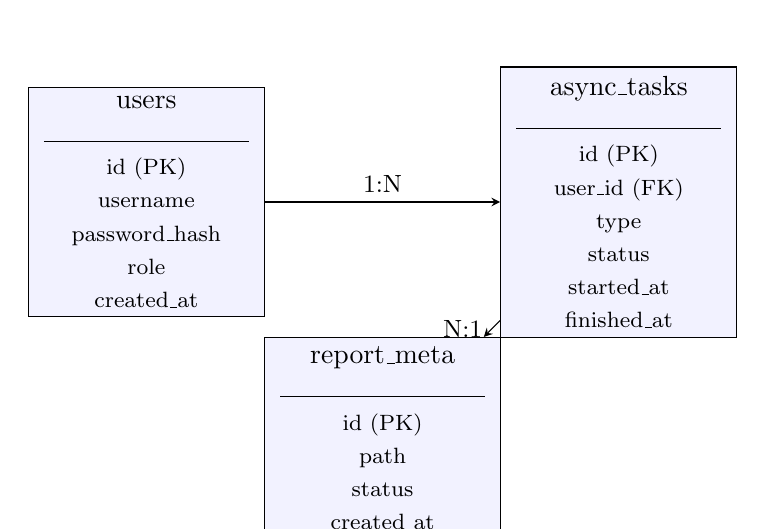
\begin{tikzpicture}[
  >=stealth,
  entity/.style={rectangle, draw, minimum width=3cm, minimum height=2.5cm, fill=blue!5, align=center},
  attr/.style={rectangle, draw, minimum width=2.5cm, minimum height=0.6cm, fill=white, font=\small, align=center},
  relation/.style={diamond, draw, fill=yellow!10, minimum width=0.8cm, minimum height=0.8cm},
]

  \node[entity] (users) at (0,0) {users\\
    \rule{2.6cm}{0.3pt}\\
    \footnotesize id (PK)\\ \footnotesize username\\ \footnotesize password\_hash\\ \footnotesize role\\ \footnotesize created\_at};
  \node[entity] (tasks) at (6,0) {async\_tasks\\
    \rule{2.6cm}{0.3pt}\\
    \footnotesize id (PK)\\ \footnotesize user\_id (FK)\\ \footnotesize type\\ \footnotesize status\\ \footnotesize started\_at\\ \footnotesize finished\_at};
  \node[entity] (reports) at (3,-3) {report\_meta\\
    \rule{2.6cm}{0.3pt}\\
    \footnotesize id (PK)\\ \footnotesize path\\ \footnotesize status\\ \footnotesize created\_at};

  \draw[->] (users) -- node[above, font=\small]{1:N} (tasks);
  \draw[->] (tasks) -- node[left, font=\small]{N:1} (reports);

\end{tikzpicture}
\caption{核心数据库ER图}
\label{fig:er}
\end{figure}

\section{核心模块详细设计}

\subsection{光伏功率预测模块}

光伏功率预测模块的设计遵循"统一输入 → 模型训练 → 物理裁剪 → 标准化输出"的管道模式。其核心类图和时序关系如图\ref{fig:prediction-pipeline}所示。

\begin{figure}[H]
\centering
\begin{tikzpicture}[
  >=stealth,
  node distance=1.5cm,
  box/.style={rectangle, draw, rounded corners, minimum width=3cm, minimum height=0.8cm, fill=blue!5, font=\small, align=center},
]

  \node[box] (data) {特征数据集 (Parquet)};
  \node[box, below of=data] (split) {时间切分\\ (train/val/test)};
  \node[box, below of=split] (train) {模型训练\\ (LightGBM/DL)};
  \node[box, below of=train] (predict) {推理预测};
  \node[box, below of=predict] (clip) {物理边界裁剪\\ \mbox{[0, cap*1.05]}};
  \node[box, below of=clip] (output) {标准预测产物\\ (CSV + 指标JSON)};

  \draw[->] (data) -- (split);
  \draw[->] (split) -- (train);
  \draw[->] (train) -- (predict);
  \draw[->] (predict) -- (clip);
  \draw[->] (clip) -- (output);
\end{tikzpicture}
\caption{预测模块管道流程图}
\label{fig:prediction-pipeline}
\end{figure}

关键设计决策包括：
\begin{enumerate}[label=(\arabic*)]
  \item \textbf{时间切分在窗口构造之前}：先按时间顺序将数据集切分为train/validation/test三段，再在各自段内构造滑动窗口。这确保了任何窗口的输入特征和目标都在同一时间段内，不会发生训练数据穿越到测试集的时间泄漏问题。
  \item \textbf{仅对训练集计算标准化参数}：对于深度学习模型，均值和标准差仅在训练集上计算，然后应用到验证集和测试集，避免验证/测试集信息通过标准化参数泄漏到训练过程中。
  \item \textbf{物理边界裁剪作为推理管道的最后一步}：无论采用何种模型，预测值在输出前必须经过$\text{clip}(x, 0, \text{capacity\_kw} \times 1.05)$操作，确保下游消费方不会接收到负功率或超容量功率值。
\end{enumerate}

\subsection{储能调度模块}

储能调度模块的设计围绕以下核心抽象展开，其类结构如图\ref{fig:dispatch-class}所示：

\begin{figure}[H]
\centering
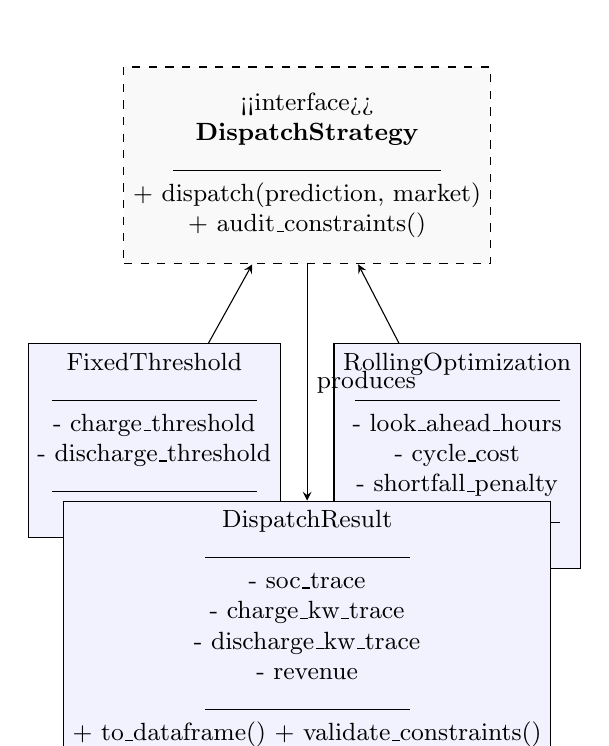
\begin{tikzpicture}[
  >=stealth,
  interface/.style={rectangle, draw, dashed, minimum width=4cm, minimum height=2.5cm, fill=gray!5, font=\small, align=center},
  class/.style={rectangle, draw, minimum width=3cm, minimum height=1.8cm, fill=blue!5, font=\small, align=center},
]

  \node[interface] (iface) at (0,0) {<<interface>>\\
    \textbf{DispatchStrategy}\\
    \rule{3.4cm}{0.3pt}\\
    + dispatch(prediction, market)\\
    + audit\_constraints()
  };

  \node[class, below left=1cm and -2cm of iface] (fixed) {FixedThreshold\\
    \rule{2.6cm}{0.3pt}\\
    - charge\_threshold\\
    - discharge\_threshold\\
    \rule{2.6cm}{0.3pt}\\
    + dispatch()
  };

  \node[class, below right=1cm and -2cm of iface] (rolling) {RollingOptimization\\
    \rule{2.6cm}{0.3pt}\\
    - look\_ahead\_hours\\
    - cycle\_cost\\
    - shortfall\_penalty\\
    \rule{2.6cm}{0.3pt}\\
    + dispatch()
  };

  \node[class, below=3cm of iface] (result) {DispatchResult\\
    \rule{2.6cm}{0.3pt}\\
    - soc\_trace\\
    - charge\_kw\_trace\\
    - discharge\_kw\_trace\\
    - revenue\\
    \rule{2.6cm}{0.3pt}\\
    + to\_dataframe()
    + validate\_constraints()
  };

  \draw[->] (fixed) -- (iface);
  \draw[->] (rolling) -- (iface);
  \draw[->] (iface) -- node[right, font=\small]{produces} (result);
\end{tikzpicture}
\caption{调度模块核心类图}
\label{fig:dispatch-class}
\end{figure}

调度决策的核心时序逻辑如下：系统首先将预测层的$t+24h$预测值按其时间戳对齐到交付时刻，然后合并来自数据层的电价和负荷市场信号，剔除市场信号缺失的交付时刻。在每个交付时刻，调度策略基于当前可用信息（当前SOC、未来预测PV、未来电价）生成充放电决策，更新SOC状态，并记录实际结算收益。在所有交付时刻遍历完成后，审计SOC越界、功率超限、同时充放电和能量守恒四项物理约束。

\subsection{策略蒸馏模块}

两阶段神经网络策略蒸馏模块的设计如图\ref{fig:distillation}所示。

\begin{figure}[H]
\centering
\begin{tikzpicture}[
  >=stealth,
  box/.style={rectangle, draw, rounded corners, minimum width=3.5cm, minimum height=0.9cm, fill=blue!5, align=center},
  teacher/.style={rectangle, draw, rounded corners, minimum width=3.5cm, minimum height=0.9cm, fill=yellow!15, align=center},
  student/.style={rectangle, draw, rounded corners, minimum width=3.5cm, minimum height=0.9cm, fill=green!10, align=center},
]

  \node[teacher] (t) at (0,-1) {教师策略\\ (滚动优化调度)};
  \node[box] (feat) at (0,0) {特征工程\\ (窗口特征、价格、SOC)};
  \node[student] (s1) at (-3.5,-3) {学生网络 Stage 1\\ 动作类型分类\\ (charge/idle/discharge)};
  \node[student] (s2) at (3.5,-3) {学生网络 Stage 2\\ 功率预测\\ (回归/分桶)};
  \node[box] (out) at (0,-5) {最终调度动作\\ (动作类型 + 功率)};

  \draw[->] (feat) -- (t);
  \draw[->] (t) -- node[left, font=\small]{标签生成} (s1);
  \draw[->] (t) -- node[right, font=\small]{标签生成} (s2);
  \draw[->] (feat) -- (s1);
  \draw[->] (feat) -- (s2);
  \draw[->] (s1) -- (out);
  \draw[->] (s2) -- (out);

  \draw[thick, dotted] (-5,-1.8) rectangle (-2,-3.8);
  \node[font=\footnotesize] at (-3.5,-4.1) {阶段一：粗分类};
  \draw[thick, dotted] (2,-1.8) rectangle (5,-3.8);
  \node[font=\footnotesize] at (3.5,-4.1) {阶段二：精细化};
\end{tikzpicture}
\caption{两阶段策略蒸馏流程图}
\label{fig:distillation}
\end{figure}

第一阶段（动作类型分类）将教师策略（Stage12滚动优化）在每个时刻的决策映射为三种离散标签。分类网络以历史PV窗口、当前SOC、市场信号和天气特征为输入，输出三分类概率分布。第二阶段细化充电或放电的具体功率值。这种两阶段设计避免了单一网络在零值（idle动作占比较大）和非零值之间分布不均导致的训练困难。

\subsection{API接口设计}

系统的RESTful API分为只读数据接口和任务提交接口两大类，核心接口如表\ref{tab:api}所示。所有接口遵循FastAPI的自动文档生成规范，响应格式统一为JSON。\cite{fastapi}

\begin{table}[H]
\centering
\caption{核心API接口列表}
\label{tab:api}
\begin{tabular}{@{}lllp{4cm}@{}}
\toprule
\textbf{方法} & \textbf{路径} & \textbf{认证} & \textbf{说明} \\
\midrule
GET  & /api/overview/summary     & JWT & 系统总览KPI数据 \\
GET  & /api/models/metrics       & JWT & 模型对比指标 \\
GET  & /api/dispatch/metrics     & JWT & 调度仿真指标 \\
GET  & /api/governance/scorecard & JWT & 策略治理评分卡 \\
GET  & /api/data/preview         & JWT & 数据预览（分页） \\
GET  & /api/reports/list         & JWT & 报告列表 \\
GET  & /api/reports/content/{id} & JWT & 报告Markdown内容 \\
GET  & /api/rawhide/report       & JWT & Rawhide电站仿真摘要 \\
GET  & /api/rawhide/dispatch-metrics & JWT & Rawhide调度指标 \\
GET  & /api/rawhide/sensitivity-metrics & JWT & Rawhide配置敏感性 \\
GET  & /api/stage21/report       & JWT & Stage21场景报告 \\
GET  & /api/stage21/dispatch-metrics & JWT & Stage21多场景调度指标 \\
POST & /api/auth/login           & 无   & 用户登录，返回JWT Token \\
POST & /api/tasks/submit         & JWT & 提交异步分析任务 \\
GET  & /api/tasks/status/{id}    & JWT & 查询任务状态 \\
\bottomrule
\end{tabular}
\end{table}

关键设计原则：（1）读接口为幂等GET请求，不触发任何计算或文件写入，只返回已存在的实验产物数据；（2）缺少实验产物时返回明确的HTTP 404响应，附带人类可读的错误消息，不静默返回空数组；（3）写接口（任务提交）为POST请求，创建异步任务并返回任务ID供轮询。

\section{本章小结}

本章从总体架构、数据库、核心模块和API接口四个层面描述了系统的设计方案。系统采用五层分层架构（数据层→预测层→调度层→治理层→展示层），各层之间通过标准化的数据产物格式（统一列名的CSV/Parquet文件）进行解耦。数据持久化采用MySQL + 文件系统混合策略。核心模块设计中强调了三个关键设计决策：时间切分先于窗口构造以防止时间泄漏、训练集专属标准化参数以避免信息泄漏、物理边界裁剪作为推理管道最后一步以保护下游消费者。API设计遵循RESTful规范，读写分离，缺失产物返回明确错误。\cite{design-patterns,fastapi}

% ============================================================
%  第五章 系统实现
% ============================================================
\chapter{系统实现}

\section{开发环境配置}

本系统的开发与实验环境配置如下：

\begin{itemize}
  \item \textbf{操作系统}：Windows 11 Pro（开发机），Ubuntu 22.04 LTS（EC2远程计算实例）
  \item \textbf{Python版本}：3.11+（兼容Anaconda Python 3.13）
  \item \textbf{深度学习环境}：PyTorch 2.0+ CPU版本（模型规模较小，无需GPU加速即可完成训练）
  \item \textbf{Node.js}：20.x LTS（前端构建）
  \item \textbf{数据库}：MySQL 8.0（开发环境），SQLite（测试环境）
  \item \textbf{版本控制}：Git，托管于本地仓库
  \item \textbf{远程计算}：AWS EC2 t3.large实例，用于HRRR大规模天气数据抽取
\end{itemize}

项目采用标准Python包结构，核心算法模块位于\texttt{src/new\_energy\_sys/}目录下，各子模块通过统一的CLI入口调用：

\begin{lstlisting}[caption={CLI入口示例}, label={lst:cli}]
# 数据准备管线
python -m new_energy_sys.cli.bootstrap_data --config configs/...
python -m new_energy_sys.cli.clean_data --config configs/...
python -m new_energy_sys.cli.build_features --config configs/...

# 模型训练与推理
python -m new_energy_sys.cli.train_baseline --config configs/...
python -m new_energy_sys.cli.run_stage9_inference --config configs/...

# 调度仿真
python -m new_energy_sys.cli.run_stage12_rolling --config configs/...
\end{lstlisting}

\section{数据采集与标准化模块实现}

数据采集模块的核心设计模式是\textbf{管道模式（Pipeline Pattern）}，将数据从原始格式到标准化特征的转换过程分解为一系列可组合的处理阶段。\cite{design-patterns}

\subsection{多源数据下载}

系统需要从PVDAQ（光伏发电数据）、NSRDB（太阳辐射数据）、OPSD（电价/负荷数据）和Open-Meteo（历史天气预报）四个公开数据源获取数据。其中，PVDAQ是NREL公开的光伏数据采集数据集，NSRDB是NREL建设的国家太阳辐射数据库，OPSD time series数据包提供欧洲电力负荷、风光出力和价格等小时级数据，Open-Meteo则提供可复用的天气API接口\cite{pvdaq-nrel,nsrdb-nrel,opsd-datapackage-2020,opsd-wiese-2019,open-meteo-2023}。数据下载的关键实现要点是\textbf{断点续传}和\textbf{速率控制}：对于大型数据文件（如NSRDB年度数据包可达数百MB），下载过程中网络中断会导致必须重新开始。为此，系统在下载前检查本地文件大小，使用HTTP Range请求实现断点续传，并设置合理的请求间隔以避免触发API速率限制。\cite{pvdaq-nrel,nsrdb-nrel,opsd-datapackage-2020,opsd-wiese-2019,open-meteo-2023}

\subsection{时间对齐与标准化}

不同数据源的时间表示格式和时区各不相同。PVDAQ使用美国山地时间（MST/MDT），NSRDB使用UTC时间，OPSD使用欧洲中部时间（CET/CEST）。标准化的核心逻辑为：\cite{pvdaq-nrel,nsrdb-nrel,opsd-wiese-2019}

\begin{lstlisting}[caption={时间标准化核心逻辑（精简自 cleaning.py）}, label={lst:time-align}]
def _standardize_timestamp(df: pd.DataFrame,
                           time_col: str,
                           source_tz: str) -> pd.DataFrame:
    """将不同数据源的时间戳统一为 UTC 小时粒度."""
    df = df.copy()
    # 解析原始时间字符串为时区感知的 datetime
    ts = pd.to_datetime(df[time_col], utc=True
                        if 'utc' in source_tz.lower() else None)
    if not ts.dt.tz:
        ts = ts.dt.tz_localize(source_tz)
    df['timestamp_utc'] = ts.dt.tz_convert('UTC')
    # 按小时取整并对齐
    df['hour_utc'] = df['timestamp_utc'].dt.floor('h')
    return df.drop(columns=[time_col])
\end{lstlisting}

该函数采用\textbf{适配器模式}的思想：每个数据源有各自的时间格式和时区，通过统一的标准化接口将其转换为UTC小时粒度，下游模块无需关心数据来源即可消费统一格式的时间戳。

\subsection{特征工程}

特征工程模块从标准化后的数据中提取三类特征：

\textbf{时间特征}：小时（0--23）、月份（1--12）、星期几（0--6）、是否周末（布尔值）。时间特征帮助模型捕捉光伏出力的日周期和季节周期规律。

\textbf{历史滑动窗口特征}：对光伏功率、GHI、DNI、温度等关键变量计算过去$N$小时（$N=1,3,6,12,24$）的滑动平均值。例如，\texttt{pv\_power\_kw\_rolling\_mean\_3h}表示过去3小时的平均光伏出力。该特征可帮助模型利用近期趋势进行预测。

\textbf{滞后目标特征}（仅训练集）：对于$t+h$预测目标，特征集中包含$t$时刻的实际光伏功率（即$y_t$）。这类特征在推理时不可用（因为推理时没有$t+h$时刻的实际值），因此系统维护\texttt{history\_only}和\texttt{weather\_history\_target\_aligned}两组特征集标签以区分生产安全特征组和离线上限特征组。

特征工程的关键设计决策是\textbf{严格按时间顺序切分}。系统在主数据集上以80/10/10的比例按时间顺序切分为训练/验证/测试集（2020-01至2021-07为训练、2021-08至2021-12为验证、2022全年为测试），然后在各自段内独立构造滑动窗口。这确保了验证集和测试集的时间戳全部晚于训练集，避免时间泄漏。

\section{光伏功率预测模块实现}

\subsection{LightGBM主模型训练}

LightGBM主模型的训练采用分层配置结构，通过JSON配置文件声明模型超参数和特征集。训练流程的核心设计模式是\textbf{模板方法模式（Template Method）}：基类定义了完整的训练→验证→测试→报告生成流程，具体模型只需实现\texttt{build\_model()}和\texttt{get\_params()}方法即可接入。\cite{lightgbm-2017,design-patterns}

\begin{lstlisting}[caption={LightGBM模型训练关键代码（精简自 tabular\_comparison.py）}, label={lst:lgbm-train}]
def train_lightgbm(X_train, y_train, X_val, y_val,
                   params: dict, feature_set_name: str):
    """训练 LightGBM 回归器，使用验证集早停."""
    model = lgb.LGBMRegressor(
        n_estimators=params.get('n_estimators', 2000),
        learning_rate=params.get('learning_rate', 0.02),
        max_depth=params.get('max_depth', 7),
        num_leaves=params.get('num_leaves', 63),
        min_child_samples=params.get('min_child_samples', 50),
        subsample=params.get('subsample', 0.8),
        colsample_bytree=params.get('colsample_bytree', 0.7),
        reg_alpha=params.get('reg_alpha', 0.1),
        reg_lambda=params.get('reg_lambda', 0.1),
        random_state=42, n_jobs=-1, verbose=-1
    )
    model.fit(
        X_train, y_train,
        eval_set=[(X_val, y_val)],
        eval_metric='rmse',
        callbacks=[lgb.early_stopping(50), lgb.log_evaluation(100)]
    )
    return model
\end{lstlisting}

设计要点：（1）\texttt{random\_state=42}固定随机种子，确保实验可复现；（2）\texttt{early\_stopping(50)}在验证集RMSE连续50轮不下降时停止训练，防止过拟合；（3）\texttt{n\_jobs=-1}利用所有CPU核心并行训练，在Windows和Linux下均正常工作。

\subsection{深度学习模型训练}

深度学习模型的训练管线统一实现在\texttt{deep\_sequence\_modeling.py}中，支持CNN-LSTM和Attention-LSTM两种架构。两种模型共享相同的训练基础设施：SmoothL1Loss损失函数（结合了L1的鲁棒性和L2的平滑性）、AdamW优化器（Adam + 解耦权重衰减）、验证集早停（patience=15）和学习率调度（ReduceLROnPlateau）。

关键实现细节：
\begin{itemize}
  \item \textbf{窗口构造与批次打包}：给定输入窗口长度$w$和目标预测步长$h$，对每个样本构造$(X[t-w:t], y[t+h])$对。使用PyTorch的DataLoader进行批次打包，\texttt{batch\_size=256}以平衡内存和训练速度。
  \item \textbf{训练集专属标准化}：在每个时间切分段内，使用训练集的均值和标准差对所有段进行z-score标准化。这确保了验证/测试集不通过标准化参数泄漏信息。
  \item \textbf{物理边界裁剪}：推理完成后，所有预测值强制裁剪到$[0, \text{capacity\_kw} \times 1.05]$范围。Persistence基线模型不需要训练，直接使用$y_t$作为$y_{t+h}$的预测。
\end{itemize}

\subsection{模型Bundling与推理固化}

Stage9推理固化的设计思想是\textbf{自包含Bundling}：将训练好的LightGBM模型对象（.pkl）、训练时使用的特征列名列表、装机容量（capacity\_kw）、训练集统计信息（均值/标准差）打包为一个完整的模型bundle，推理时通过统一的\texttt{predict\_with\_bundle()}接口加载和消费。

\begin{lstlisting}[caption={模型Bundle推理接口（精简自 stage9\_inference.py）}, label={lst:bundle}]
def predict_with_bundle(bundle: dict, X: pd.DataFrame) -> np.ndarray:
    """使用 model bundle 推理，强制执行特征校验和物理边界裁剪."""
    model = bundle['model']
    expected_cols = bundle['feature_columns']
    capacity_kw = bundle['capacity_kw']

    # 1. 特征列一致性校验
    missing = set(expected_cols) - set(X.columns)
    extra = set(X.columns) - set(expected_cols)
    if missing or extra:
        raise ValueError(f"Feature mismatch: missing={missing}, extra={extra}")

    # 2. 按顺序选取特征列
    X_ordered = X[expected_cols]

    # 3. 数值校验: 无缺失值, 无无穷值
    assert not X_ordered.isnull().any().any(), "NaN in features"
    assert np.isfinite(X_ordered.values).all(), "Inf in features"

    # 4. 推理
    raw_pred = model.predict(X_ordered)

    # 5. 物理边界裁剪
    return np.clip(raw_pred, 0.0, capacity_kw * 1.05)
\end{lstlisting}

这种Bundle设计的优势在于：提供完整的推理自检（特征列、缺失值、无穷值），强制物理边界裁剪，且Bundle对象可独立分发——消费方无需知道模型类型（LightGBM或深度学习），只需调用统一接口。

\section{储能调度模块实现}

\subsection{固定阈值与策略敏感性分析}

固定阈值策略的核心实现是一个状态机：维护当前SOC状态，按时间顺序遍历每个交付时刻，根据预测PV、电价和当前SOC决定充放电动作，更新SOC并记录收益。策略敏感性分析在此基础上对电价分位数网格进行扫描，对每组（充电阈值分位数, 放电阈值分位数）组合运行完整的年度调度仿真，输出所有候选策略的收益、充放电量、循环次数和约束审计结果。

\begin{lstlisting}[caption={固定阈值调度核心逻辑（精简自 storage.py）}, label={lst:dispatch}]
def dispatch_fixed_threshold(
    predictions: pd.DataFrame,
    price_series: pd.Series,
    charge_threshold: float,
    discharge_threshold: float,
    soc_min: float = 0.1,
    soc_max: float = 0.9,
    efficiency: float = 0.90,
    capacity_kwh: float,
    max_charge_kw: float,
    max_discharge_kw: float
) -> pd.DataFrame:
    """固定阈值储能调度仿真."""
    soc = soc_min * capacity_kwh  # 初始 SOC
    results = []

    for _, row in predictions.iterrows():
        price = price_series.get(row['delivery_hour'], None)
        if price is None:
            continue  # 缺少市场信号，跳过

        pred_kw = row['prediction_kw']
        charge_kw = discharge_kw = 0.0

        if pred_kw > 0 and price < charge_threshold and soc < soc_max * capacity_kwh:
            charge_kw = min(pred_kw, max_charge_kw,
                            (soc_max * capacity_kwh - soc) / efficiency)
        elif price > discharge_threshold and soc > soc_min * capacity_kwh:
            discharge_kw = min(max_discharge_kw, (soc - soc_min * capacity_kwh) * efficiency)

        soc += charge_kw * efficiency - discharge_kw / efficiency
        results.append({...})

    return pd.DataFrame(results)
\end{lstlisting}

调度输出的设计模式是\textbf{自审计（Self-Auditing）}：每次仿真完成后，系统自动运行SOC越界、功率超限、同时充放电和能量守恒四项检查，将审计结果写入指标的\texttt{quality\_gates}字段。这确保任何消费调度结果的模块（治理层、展示层、论文）都能立即确认其物理合理性。\cite{bess-review-2023,milp-dispatch-2021}

\subsection{滚动优化调度}

Stage12滚动优化调度的核心创新在于\textbf{退化策略（Fallback Strategy）}设计。系统最初尝试实现逐小时SOC离散动态规划——将SOC从0.1到0.9以0.01为步长离散为81个状态，在每个交付时刻对当前状态求解未来24小时的最优充放电路径。但该方法在三年小时级样本（约25,000个交付时刻）上每次求解都需遍历81×3（SOC状态×动作=充电/放电/空闲）的状态-动作空间，单次运行超过120秒并触发超时。\cite{bo-two-stage-rolling-2025,li-mpc-microgrid-2025,design-patterns}

经过复盘，系统将方法改为\textbf{快速24小时前瞻价差策略}：在每个交付时刻扫描未来24小时的电价序列，寻找最大正价差窗口（低电价区间充电、高电价区间放电），同时计入循环成本（EUR/kWh）、短缺惩罚和SOC终端稳定约束。该方法的时间复杂度为$O(T \times H)$（$T$为总交付时刻数，$H=24$为前瞻窗口），在25,000个交付时刻上可在30秒内完成，远优于DP的指数级复杂度。\cite{bo-two-stage-rolling-2025,li-mpc-microgrid-2025,drl-energy-storage-2023}

\subsection{两阶段神经网络策略蒸馏}

Stage20B两阶段策略蒸馏是系统的深度学习调度核心。教师调度轨迹定义如式\ref{eq:teacher-trajectory}所示，其中每个样本由特征向量、动作类型和动作功率组成。\cite{policy-distillation-2016}

\begin{equation}
\mathcal{D} = \{(\mathbf{x}_t, a_t^{\text{type}}, a_t^{\text{power}})\}_{t=1}^{T}
\label{eq:teacher-trajectory}
\end{equation}

动作类型与动作功率的取值范围如式\ref{eq:action-domain}所示，动作类型0、1、2分别对应充电、空闲和放电三类调度状态。

\begin{equation}
a_t^{\text{type}} \in \{0,1,2\}, \qquad a_t^{\text{power}} \in \mathbb{R}_{\ge 0}
\label{eq:action-domain}
\end{equation}

学生网络由动作类型分类网络和功率细化网络组成，其映射关系如式\ref{eq:student-networks}所示。

\begin{equation}
f_{\text{stage1}}: \mathbf{x}_t \mapsto a_t^{\text{type}}, \qquad
f_{\text{stage2}}: \mathbf{x}_t \mapsto a_t^{\text{power}}
\label{eq:student-networks}
\end{equation}

在线推理阶段，系统先由第一阶段网络判断动作类型，再由第二阶段网络输出功率桶或功率估计值，其推理过程如式\ref{eq:distillation-inference}所示。完整算法描述如算法\ref{alg:distillation}所示。

\begin{equation}
\hat{a}_t^{\text{type}} = f_{\text{stage1}}(\mathbf{x}_t), \qquad
\hat{p}_t = f_{\text{stage2}}(\mathbf{x}_t)
\label{eq:distillation-inference}
\end{equation}

\begin{algorithm}[H]
\caption{两阶段神经网络策略蒸馏}
\label{alg:distillation}
\begin{algorithmic}[1]
\Require 教师调度轨迹$\mathcal{D}$（见式\ref{eq:teacher-trajectory}），动作取值范围见式\ref{eq:action-domain}
\Ensure 学生网络$f_{\text{stage1}}(\cdot)$与$f_{\text{stage2}}(\cdot)$（见式\ref{eq:student-networks}）

\State \textbf{// 阶段一：动作类型分类}
\State 从 $\mathcal{D}$ 提取分类数据集 $\{(\mathbf{x}_t, a_t^{\text{type}})\}$
\State 训练三分类MLP $f_{\text{stage1}}: \mathbf{x} \mapsto \{\text{charge}, \text{idle}, \text{discharge}\}$
\State 使用交叉熵损失 + 类别权重平衡

\State \textbf{// 阶段二：功率细化}
\State 从 $\mathcal{D}$ 筛选 $a_t^{\text{type}} = \text{discharge}$ 的样本
\State 将连续放电功率离散化为 $K$ 个桶（按分位数断点）
\State 训练 $K$ 类分类MLP $f_{\text{stage2}}: \mathbf{x} \mapsto$ 功率桶标签

\State \textbf{// 策略推理：物理回放仿真}
\For{$t = 1$ to $T$}
    \State $\hat{a}_{\text{type}} \gets f_{\text{stage1}}(\mathbf{x}_t)$
    \If{$\hat{a}_{\text{type}} = \text{discharge}$}
        \State $\hat{p}_{\text{bucket}} \gets f_{\text{stage2}}(\mathbf{x}_t)$
        \State $\hat{p} \gets$ 桶中心值
    \Else
        \State $\hat{p} \gets 0$
    \EndIf
    \State 应用物理约束：$\hat{p} \gets \min(\hat{p}, \text{当前可用放电功率})$
    \State 更新电池SOC状态
\EndFor
\State \Return 学生策略的完整调度轨迹
\end{algorithmic}
\end{algorithm}

该算法的\textbf{策略模式（Strategy Pattern）}体现在教师策略的可替换性：Stage20B以Stage12滚动优化为首步决策教师，但任何产生充放电离散动作和功率标签的调度策略均可作为教师。两阶段分类设计将稀疏的动作空间（idle占比高、充电和放电稀疏）分解为粗粒度的动作类型判断和细粒度的功率选择，有效避免了单阶段多分类的训练不稳定问题。\cite{policy-distillation-2016,design-patterns}

\section{电池退化模块实现}

电池退化模块基于\textbf{雨流计数法（Rainflow Counting）} 对电池SOC时间序列进行循环识别。雨流计数的核心思想是将SOC曲线视为材料应力-应变曲线，识别其中的"full cycle"和"half cycle"——将SOC从波峰下降到波谷再回到波峰的封闭回路计为一个完整循环，将孤立的上升或下降段计为半循环。\cite{rainflow-soc-2022}

每个识别出的循环按其循环深度（Depth of Discharge, DoD）和平均SOC查表获得对应的SOH消耗量，累加到总SOH衰减中。电池健康状态的衰减模型为：\cite{battery-degradation-review-2021,rainflow-soc-2022}

\begin{equation}
\text{SOH}_{t+1} = \text{SOH}_{t} - \sum_{c \in \text{cycles}(t)} \delta_{\text{SOH}}(\text{DoD}_c, \overline{\text{SOC}}_c)
\label{eq:soh}
\end{equation}

其中 $\delta_{\text{SOH}}(\cdot)$ 为查表函数，基于文献中常见的磷酸铁锂（LFP）电池循环寿命数据构建。

\section{可视化展示模块实现}

\subsection{前端架构}

前端采用Vue 3组合式API（Composition API）的\texttt{<script setup>}语法糖，基于模块化分层结构组织：\cite{vue3}

\begin{itemize}
  \item \texttt{services/} —— API调用封装层，每个service对应后端一个功能模块（overviewService、modelService、dispatchService等），统一处理axios请求和错误；
  \item \texttt{charts/} —— 纯函数图表option生成器，接收数据返回ECharts配置对象，不包含Vue组件逻辑；
  \item \texttt{components/} —— 共享UI组件（PageState通用状态组件、MetricGrid指标卡片、ChartCard图表容器、PageSection分区组件）；
  \item \texttt{views/} —— 页面级组件（OverviewDashboard、ModelComparison、DispatchSimulation、GovernanceAnalysis、DataExplorer、ReportViewer）。
\end{itemize}

这种分层结构体现了\textbf{关注点分离（Separation of Concerns）}原则：数据获取（services）、数据到视图的映射（charts/utils）和UI渲染（components/views）各司其职。\cite{design-patterns,vue3}

\subsection{通用页面状态管理}

前端实现了一个通用\texttt{PageState}组件，统一管理页面的加载、错误、空数据和重试四种状态：

\begin{lstlisting}[caption={PageState.vue 核心逻辑}, label={lst:pagestate}]
<template>
  <div v-if="loading" class="page-state">
    <el-skeleton :rows="8" animated />
  </div>
  <div v-else-if="error" class="page-state">
    <el-result icon="error" :title="error" :sub-title="errorDetail">
      <template #extra>
        <el-button type="primary" @click="$emit('retry')">重试</el-button>
      </template>
    </el-result>
  </div>
  <div v-else-if="empty" class="page-state">
    <el-result icon="info" title="暂无数据" :sub-title="emptyMessage" />
  </div>
  <slot v-else />
</template>
\end{lstlisting}

该组件的设计使得每个页面可以声明式地切换四种状态，无需在每个页面中重复编写骨架屏和错误弹窗逻辑。

\subsection{主要功能界面展示}

系统登录界面如图\ref{fig:frontend-login}所示。登录页由\texttt{Login.vue}实现，前端不在页面中展示明文演示账号，而是通过统一认证接口提交用户凭据；认证成功后，前端会写入会话状态并进入系统总览页。

\begin{figure}[H]
  \centering
  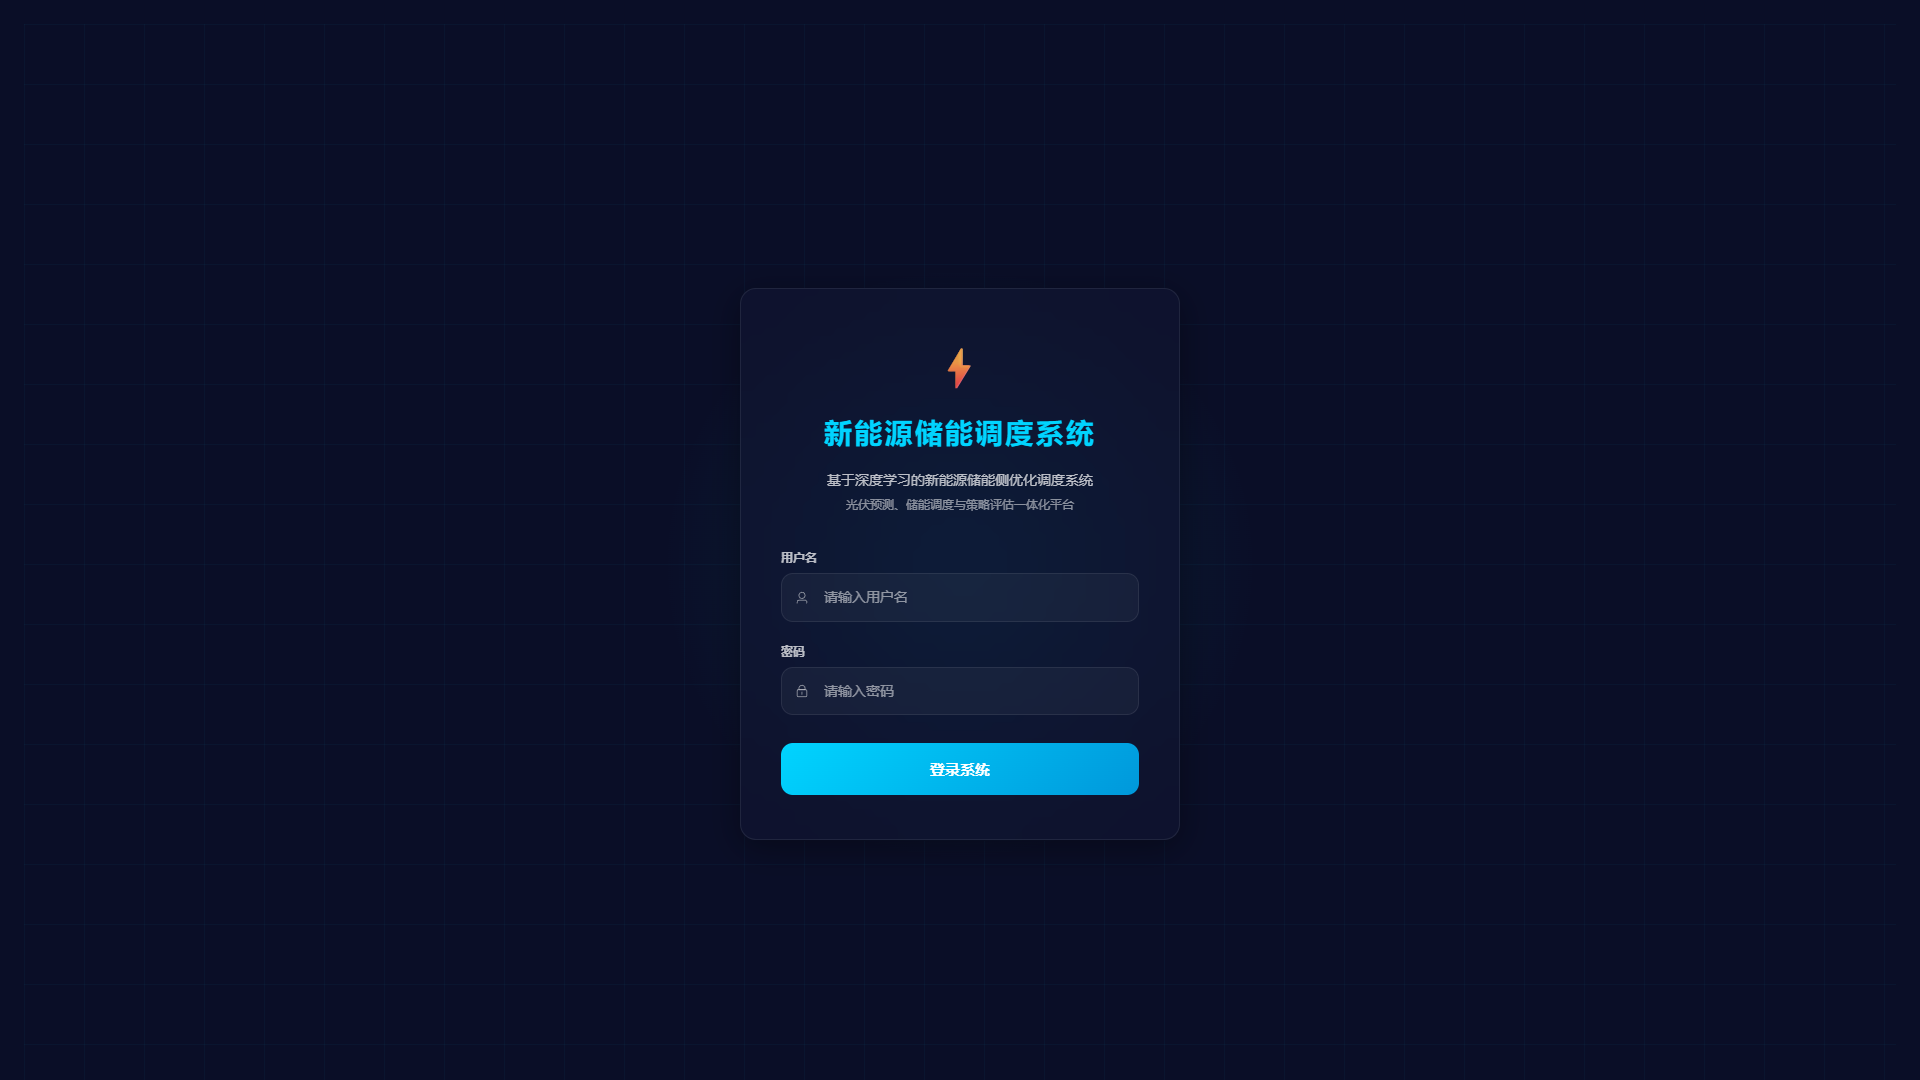
\includegraphics[width=0.92\textwidth]{figures/frontend/frontend_login.png}
  \caption{系统登录界面}
  \label{fig:frontend-login}
\end{figure}

系统总览界面如图\ref{fig:frontend-overview}所示。该页面由\texttt{OverviewDashboard.vue}实现，用于集中展示项目概况、核心指标、预测效果概览和主要功能入口，使用户进入系统后能够快速了解当前数据覆盖周期、主模型口径和调度收益边界。

\begin{figure}[H]
  \centering
  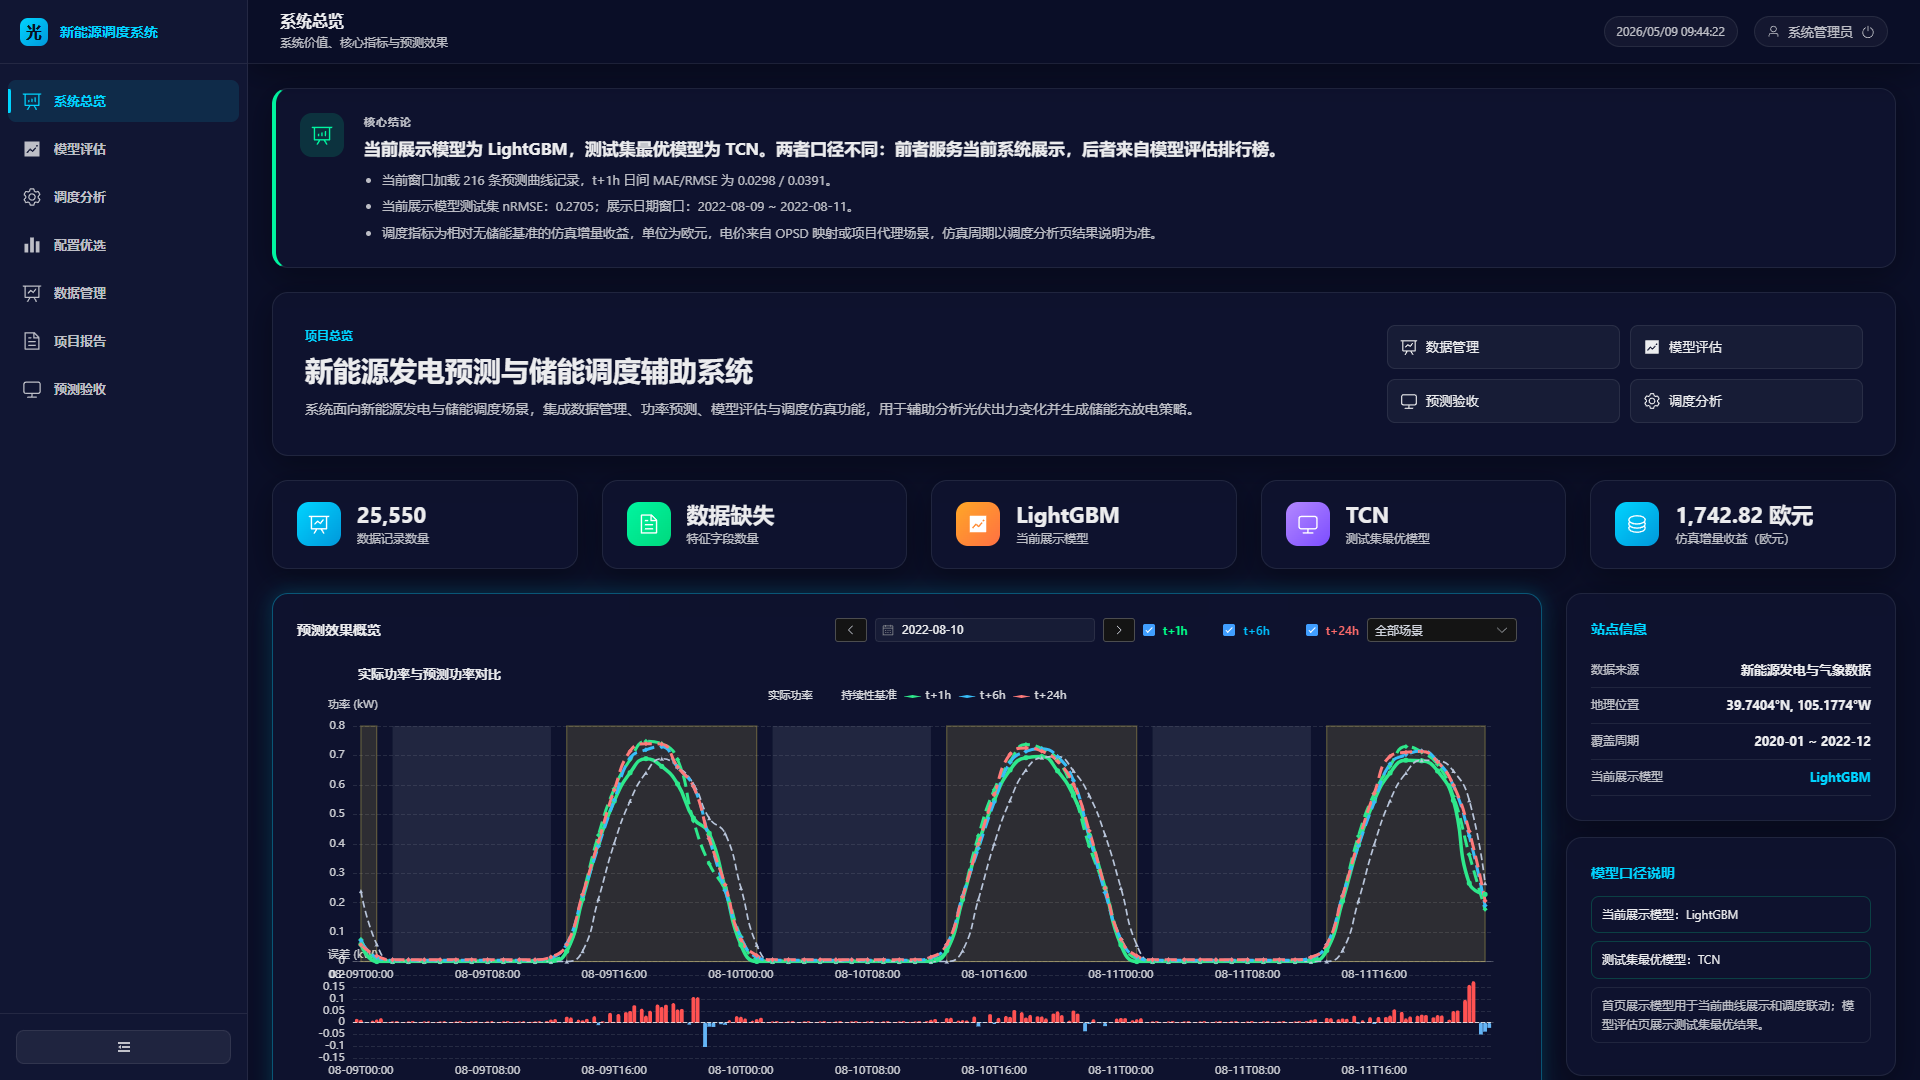
\includegraphics[width=0.92\textwidth]{figures/frontend/frontend_overview.png}
  \caption{系统总览界面}
  \label{fig:frontend-overview}
\end{figure}

模型评估与排行榜界面如图\ref{fig:frontend-models}所示。该页面由\texttt{ModelComparison.vue}实现，主要展示不同预测模型在统一测试集上的评价指标，使LightGBM主模型、TCN和其他深度学习对比模型能够在同一页面中进行横向比较。

\begin{figure}[H]
  \centering
  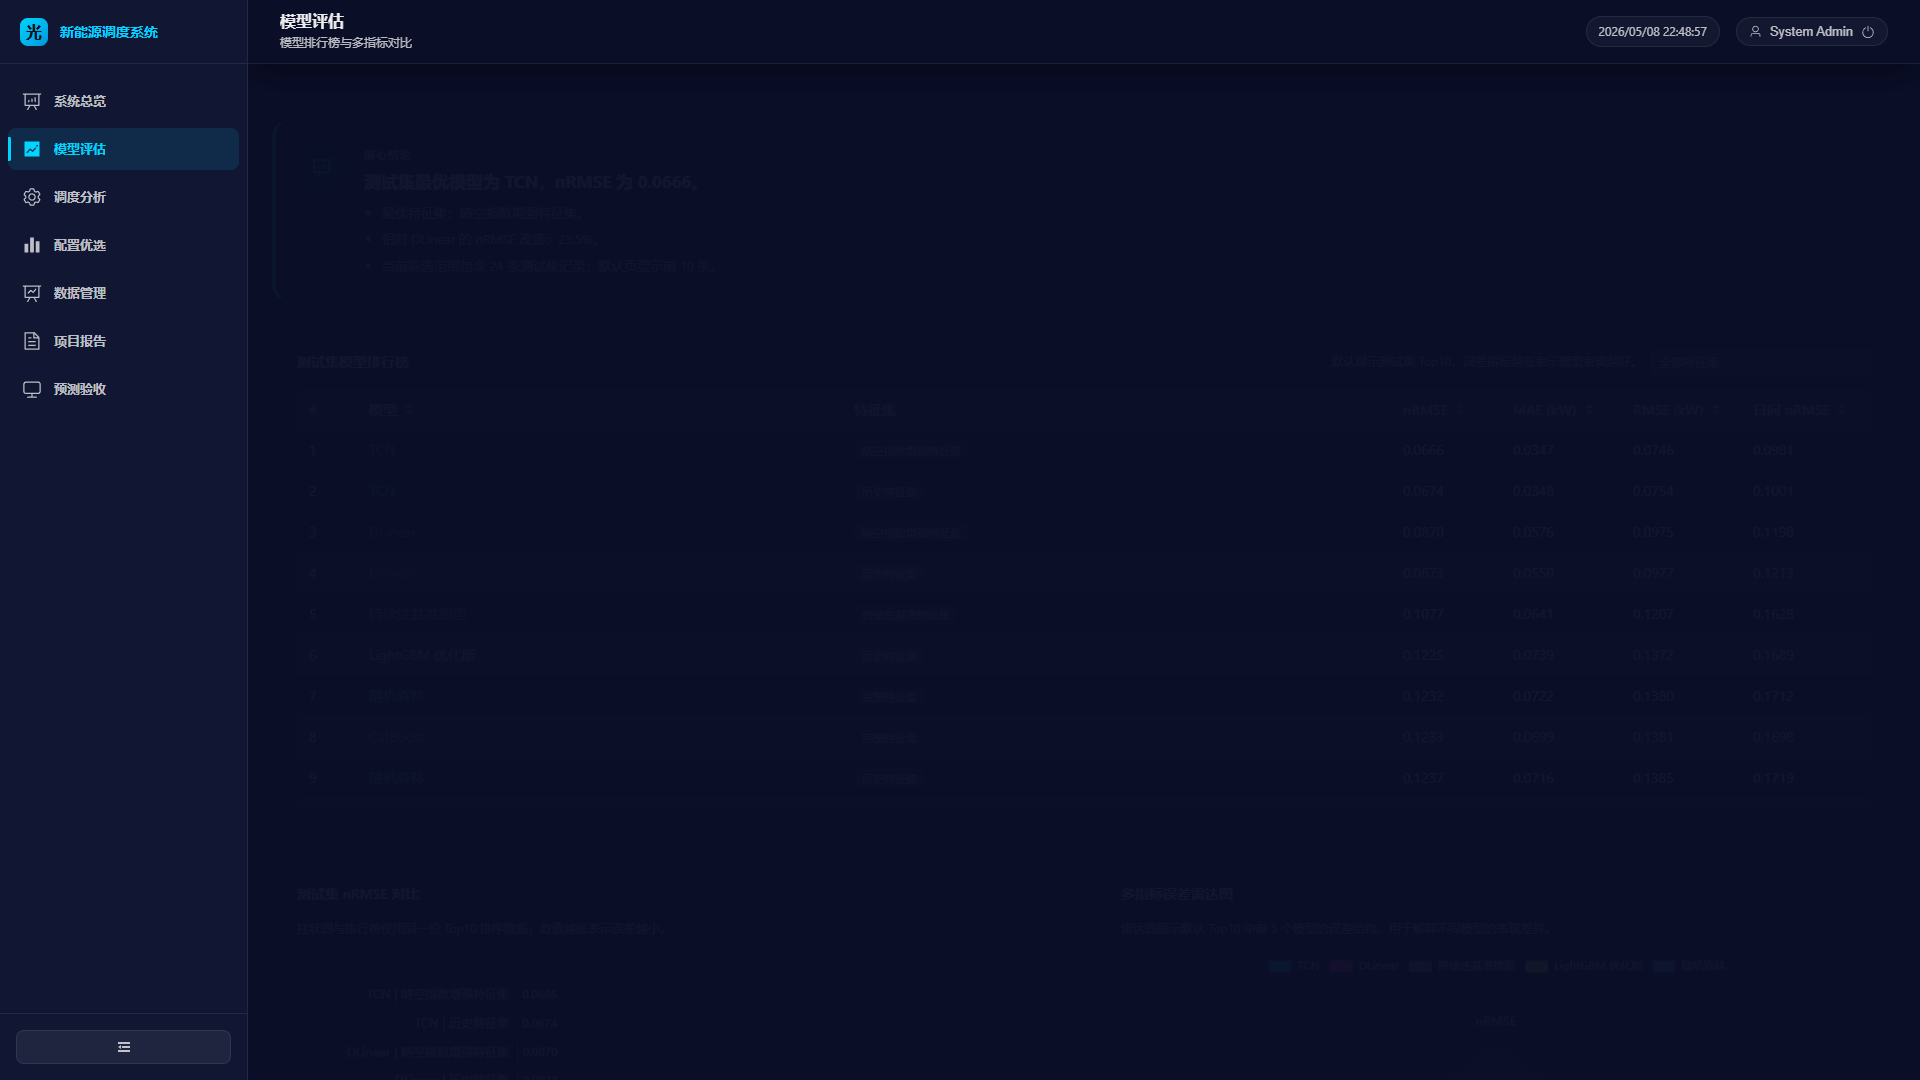
\includegraphics[width=0.92\textwidth]{figures/frontend/frontend_models.png}
  \caption{模型评估与排行榜界面}
  \label{fig:frontend-models}
\end{figure}

实时天气驱动调度实验界面如图\ref{fig:frontend-dispatch-stage21}所示。该页面由\texttt{DispatchSimulation.vue}承载，默认展示“天气驱动实验台”页签，用户可调整天气场景、电价场景、优化目标和储能参数，并查看后端返回的天气、光伏预测、SOC、功率调度和收益指标。页面顶部保留“仿真边界”提示，明确该结果为天气驱动和价格场景下的参考仿真，不是Rawhide真实结算收益。

\begin{figure}[H]
  \centering
  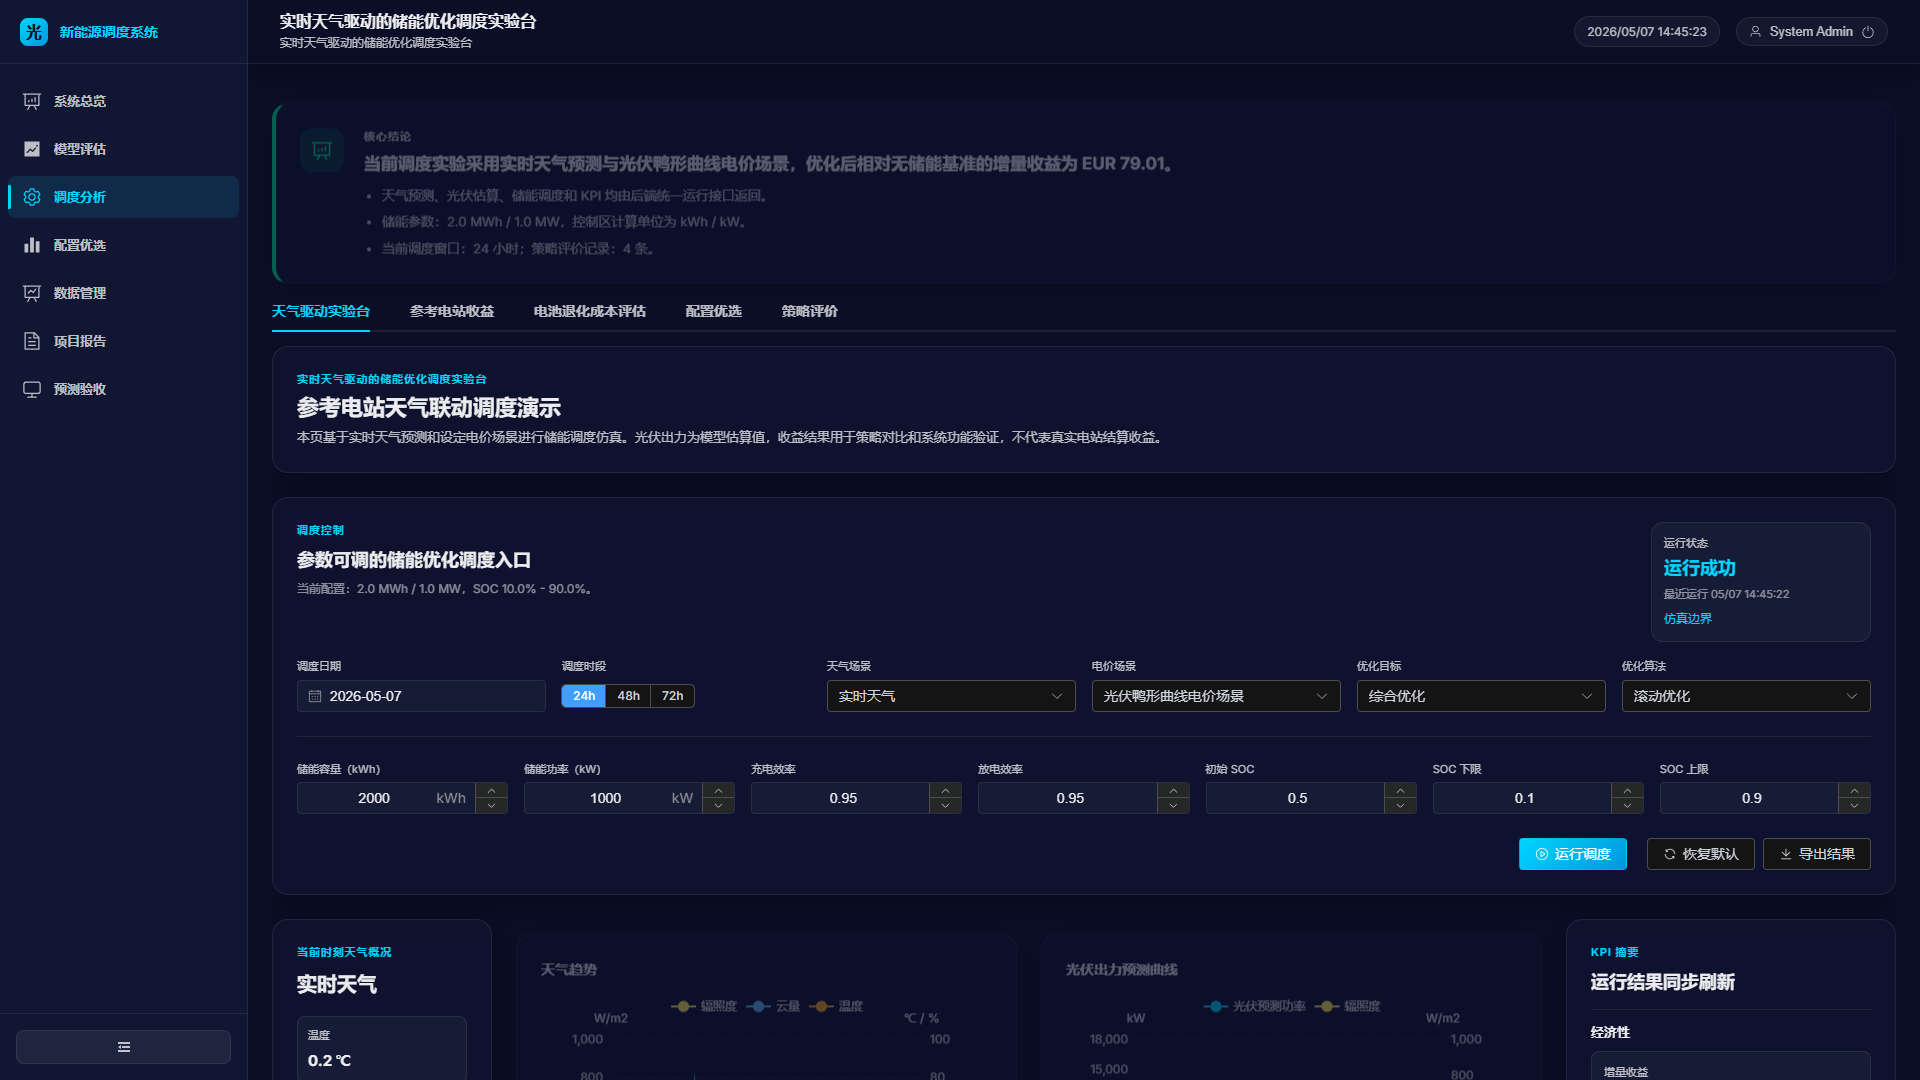
\includegraphics[width=0.92\textwidth]{figures/frontend/frontend_dispatch_stage21.png}
  \caption{实时天气驱动调度实验界面}
  \label{fig:frontend-dispatch-stage21}
\end{figure}

储能配置治理界面如图\ref{fig:frontend-governance}所示。该页面由\texttt{GovernanceAnalysis.vue}实现，面向Stage15配置敏感性分析结果，展示容量、功率、目标函数惩罚项和Pareto推荐边界，辅助用户理解不同储能配置对收益和运行质量的影响。

\begin{figure}[H]
  \centering
  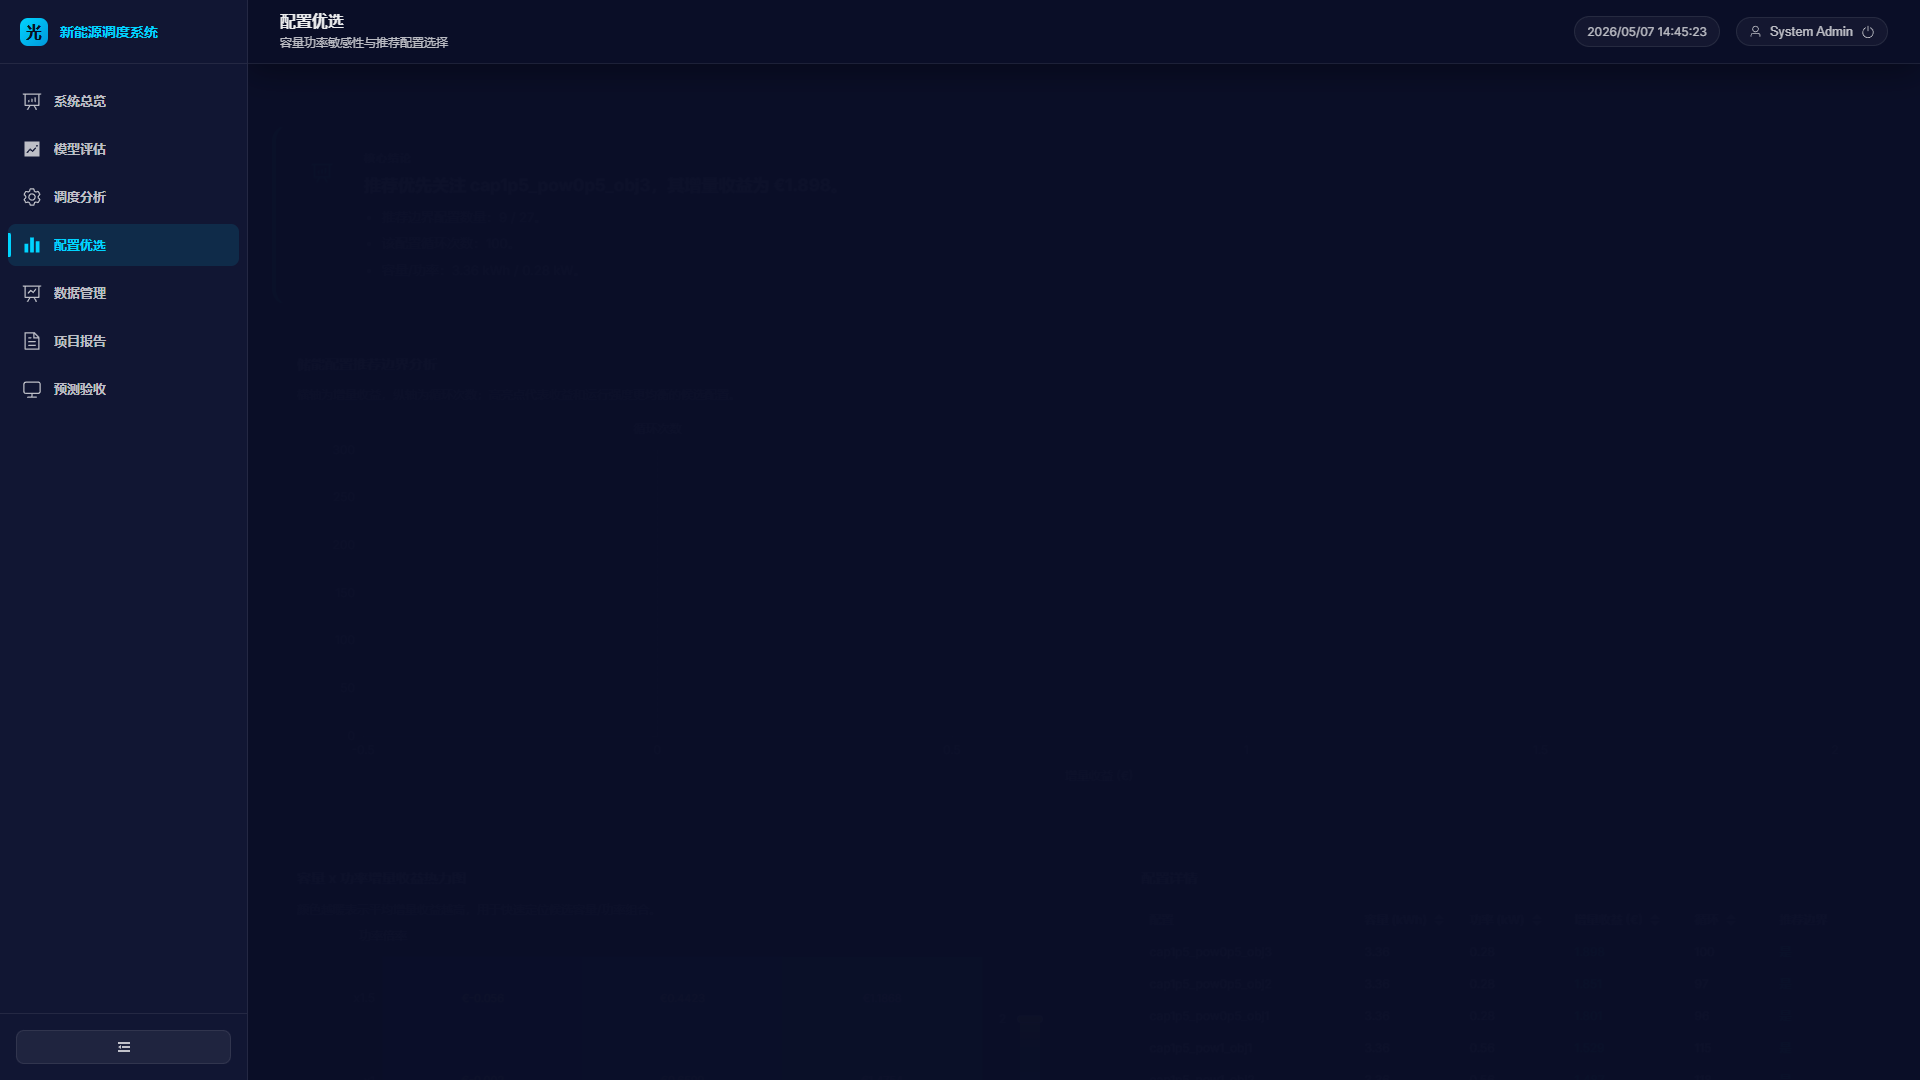
\includegraphics[width=0.92\textwidth]{figures/frontend/frontend_governance.png}
  \caption{储能配置治理界面}
  \label{fig:frontend-governance}
\end{figure}

数据管理与特征分析界面如图\ref{fig:frontend-data}所示。该页面由\texttt{DataExplorer.vue}实现，用于展示数据质量、特征重要性和任务命令入口，帮助用户从数据侧追踪预测模型输入变量及其相对贡献。

\begin{figure}[H]
  \centering
  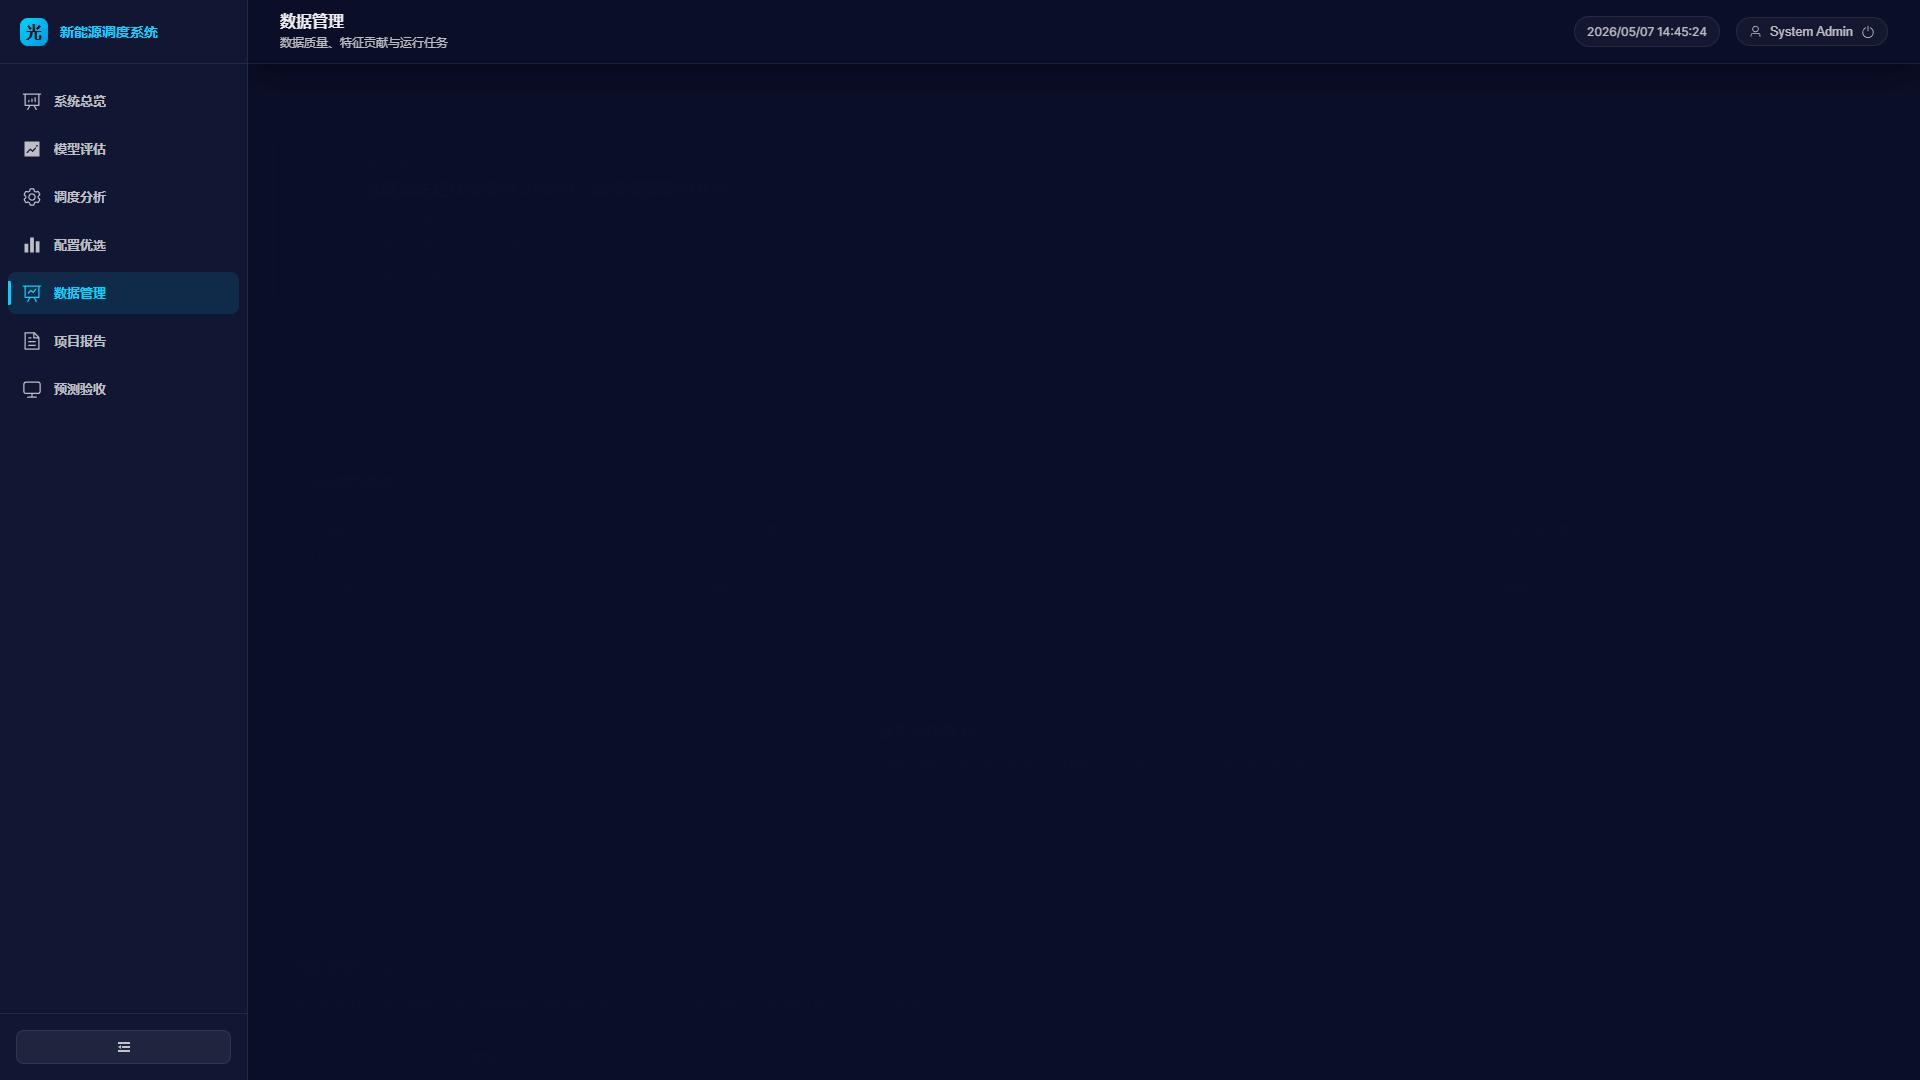
\includegraphics[width=0.92\textwidth]{figures/frontend/frontend_data.png}
  \caption{数据管理与特征分析界面}
  \label{fig:frontend-data}
\end{figure}

\subsection{安全加固}

生产化安全整改中实现了四个关键安全措施：（1）Markdown渲染内容通过\texttt{DOMPurify.sanitize()}清洗后再注入；（2）生产环境JWT签名密钥通过环境变量\texttt{NES\_JWT\_SECRET}强制配置，使用默认值时拒绝启动；（3）CORS白名单通过环境变量显式指定，拒绝\texttt{*}通配符；（4）登录页面不展示任何demo明文凭据。这些措施解决了OWASP Top 10中的跨站脚本（XSS）、身份认证失效和跨站请求伪造等安全风险。\cite{dompurify,jwt-rfc7519,owasp-top10-2021}

\section{设计模式与优秀实践总结}

本系统在实现过程中应用了以下设计模式和优秀实践：

\begin{enumerate}[label=(\arabic*)]
  \item \textbf{管道模式（Pipeline Pattern）}：数据采集→标准化→清洗→特征工程→模型训练→推理→调度，每阶段通过标准化产物格式解耦，下游模块只需遵守输入格式契约即可独立开发和测试。\cite{design-patterns}
  \item \textbf{模板方法模式（Template Method）}：预测模型的训练流程（数据切分→训练→验证→测试→报告）由基类固化，具体模型只需实现子步骤，新增模型无需重复编写管道逻辑。\cite{design-patterns}
  \item \textbf{策略模式（Strategy Pattern）}：调度策略通过\texttt{DispatchStrategy}抽象接口统一消费，不同策略（固定阈值、滚动优化、策略蒸馏）可互换对比，新增策略无需修改治理层和展示层。\cite{design-patterns}
  \item \textbf{自审计模式（Self-Auditing）}：每次调度仿真完成后自动运行SOC、功率、能量守恒等多维物理约束检查，审计结果随指标一同输出，确保所有消费方都能获得物理可行性证明。
  \item \textbf{自包含Bundle模式}：模型Bundle打包了模型对象、特征列名、容量参数和统计信息，推理方无需了解模型类型即可安全消费。
  \item \textbf{门禁驱动质量保证（Gate-Driven QA）}：每个Stage的实验输出都经过硬性质量门禁验证（如特征非空、时间戳单调、物理约束通过等），门禁清单写入报告的JSON/Markdown产物中。
\end{enumerate}

\section{本章小结}

本章详述了系统各核心模块的实现细节。数据层采用管道模式和适配器模式处理多源异构数据，预测层通过LightGBM模板方法和深度学习统一训练管线实现多模型对比，调度层从固定阈值演进到滚动优化和两阶段策略蒸馏，前端通过关注点分离和通用状态管理实现健壮的用户界面。特别总结了六种贯穿系统的设计模式，这些模式的运用使得系统在保持各模块独立可测的同时实现了灵活的组合和演进。

% ============================================================
%  第六章 系统测试与分析
% ============================================================
\chapter{系统测试与分析}

\section{测试环境}

系统的测试分为后端Python单元测试、前端静态检查和E2E自动化测试三个层次，测试环境配置如下：

\begin{itemize}
  \item Python单元测试：pytest 8.x，运行于开发机Windows 11 + Anaconda Python 3.13
  \item 前端静态检查：ESLint + 自定义\texttt{static-check.mjs}脚本（检查各页面Vue组件是否包含错误态和边界提示）
  \item 前端E2E测试：Playwright 1.x，使用系统Chrome/Edge浏览器
  \item API契约测试：自定义Python脚本\texttt{api\_smoke\_frontend\_contract.py}
  \item CI环境：GitHub Actions（最小CI，运行核心Python单测+前端静态检查）
\end{itemize}

\section{功能测试}

\subsection{后端单元测试}

核心调度模块和Stage21市场场景模块的单元测试覆盖了以下关键场景：

\begin{table}[H]
\centering
\caption{后端单元测试用例及结果}
\label{tab:unit-tests}
\begin{tabular}{@{}llc@{}}
\toprule
\textbf{测试模块} & \textbf{测试用例} & \textbf{结果} \\
\midrule
\multirow{4}{*}{test\_storage\_dispatch\_core.py}
  & SOC初始化在合法范围内 & 通过 \\
  & 充电不超过SOC上限 & 通过 \\
  & 放电不低于SOC下限 & 通过 \\
  & 能量守恒一致性验证 & 通过 \\
  & 同一时刻不出现同时充放电 & 通过 \\
\midrule
\multirow{4}{*}{test\_stage21\_market\_scenarios.py}
  & 5类价格场景全部生成成功 & 通过 \\
  & flat\_proxy\_30场景值恒为30 EUR/MWh & 通过 \\
  & tou\_peak\_valley场景符合峰谷价差 & 通过 \\
  & solar\_duck\_curve场景午间低于早晚 & 通过 \\
  & 所有场景is\_real\_settlement\_price=false & 通过 \\
\bottomrule
\end{tabular}
\end{table}

全部9个单元测试用例均通过（\texttt{pytest -q}：9 passed）。

\subsection{API契约测试}

API烟雾测试脚本\texttt{api\_smoke\_frontend\_contract.py}对全部12个关键接口进行了冒烟测试，覆盖登录认证、只读数据接口和Stage21新接口。测试结果：全部12个接口返回HTTP 200（正常）或404（缺少产物时的正确错误响应），无500错误。

\subsection{前端E2E测试}

Playwright E2E测试覆盖以下场景，重点验证路由、移动端布局和DOMPurify清洗后的Markdown渲染安全性\cite{dompurify}：

\begin{table}[H]
\centering
\caption{E2E测试用例}
\label{tab:e2e}
\begin{tabular}{@{}llc@{}}
\toprule
\textbf{用例} & \textbf{验证内容} & \textbf{结果} \\
\midrule
登录页 & 不展示明文demo凭据 & 通过 \\
admin登录 & 使用环境变量注入凭据登录成功 & 通过 \\
路由导航 & 6个核心页面均可访问 & 通过 \\
移动端布局 & 320px视口下页面无横向溢出 & 通过 \\
Markdown XSS & DOMPurify清洗后无脚本注入 & 通过 \\
权限错误 & guest提交任务后显示权限错误提示 & 通过 \\
\bottomrule
\end{tabular}
\end{table}

全部6个E2E测试用例均通过（\texttt{npm run test:e2e}：6 passed）。

预测验收界面如图\ref{fig:frontend-inspect}所示。该页面由\texttt{InspectionDashboard.vue}实现，E2E测试会验证预测验收图表画布已经真实渲染，并通过前一天、后一天和场景筛选等控件检查页面交互是否正常。

\begin{figure}[H]
  \centering
  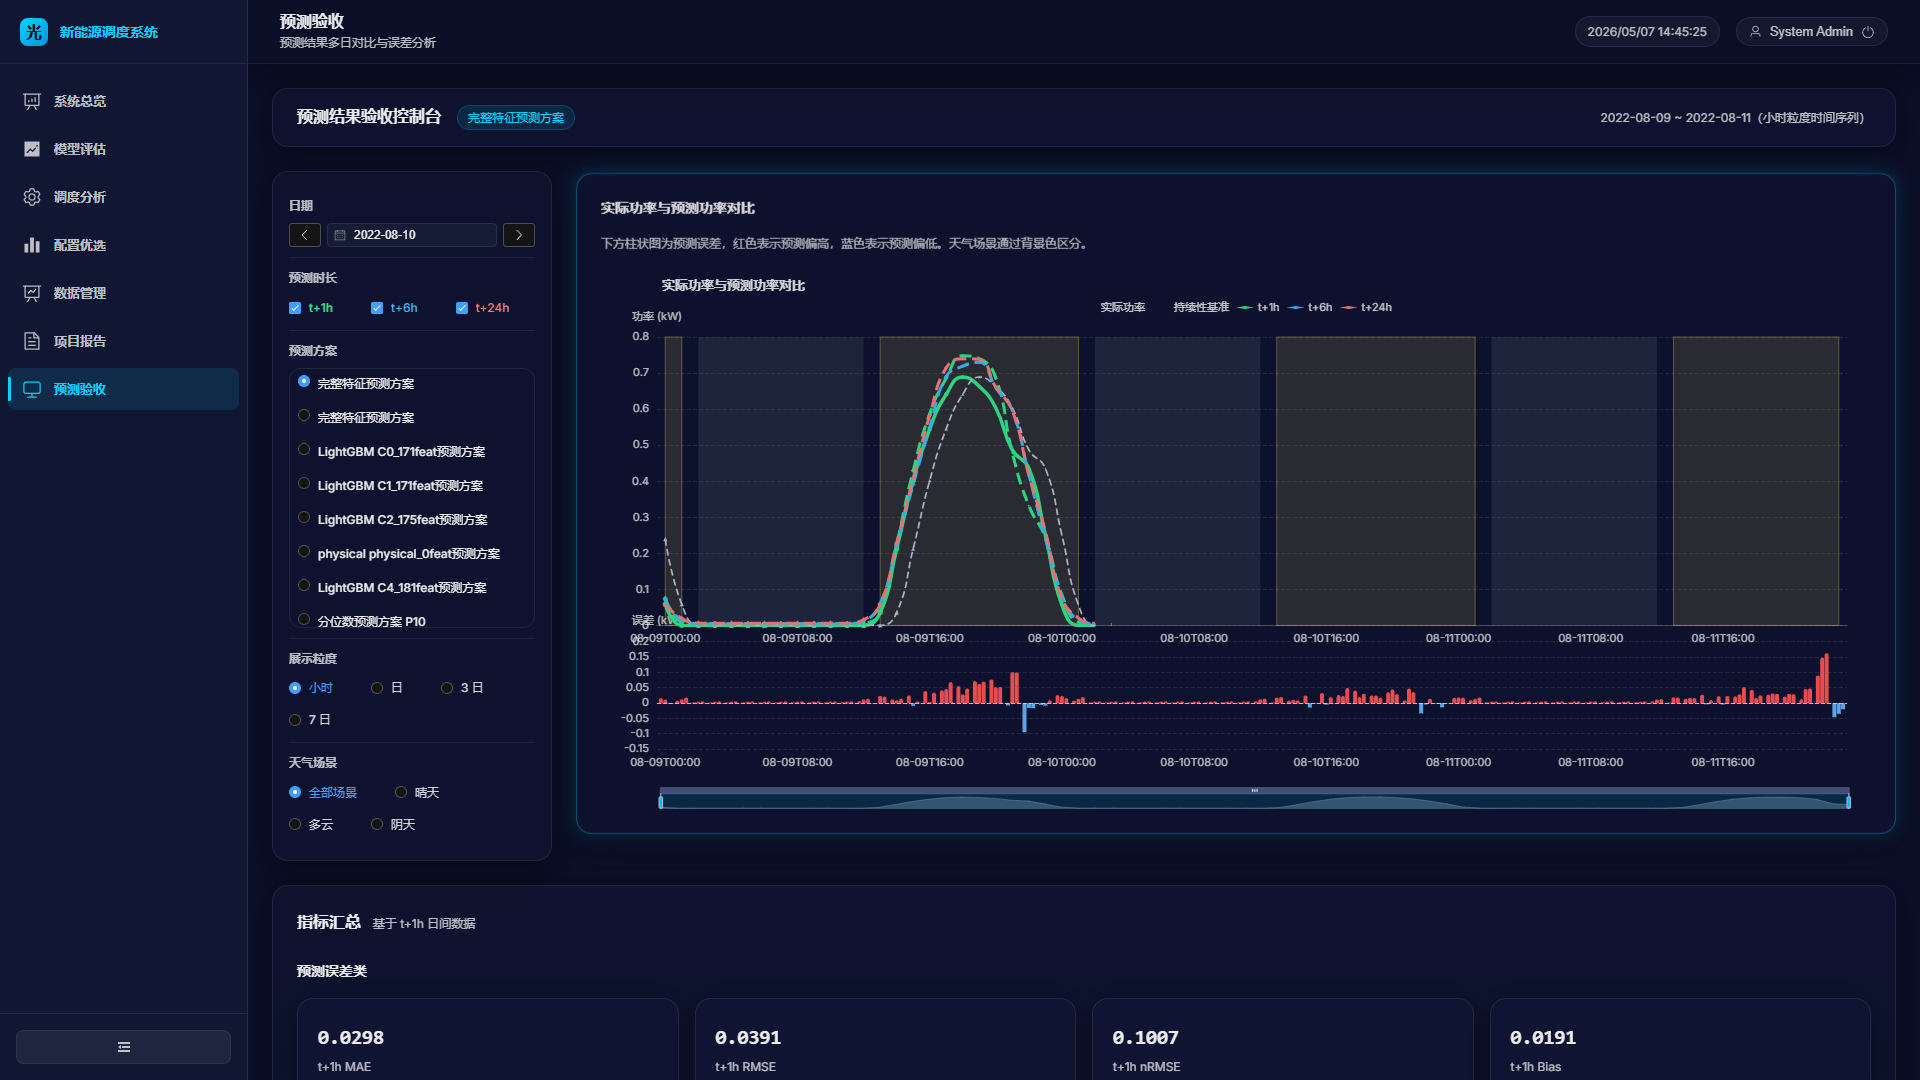
\includegraphics[width=0.92\textwidth]{figures/frontend/frontend_inspect.png}
  \caption{预测验收界面}
  \label{fig:frontend-inspect}
\end{figure}

项目报告浏览界面如图\ref{fig:frontend-reports}所示。该页面由\texttt{ReportViewer.vue}实现，测试重点包括报告列表加载、Markdown正文渲染、DOMPurify安全清洗和表格内容展示，确保阶段报告能够在前端安全浏览。

\begin{figure}[H]
  \centering
  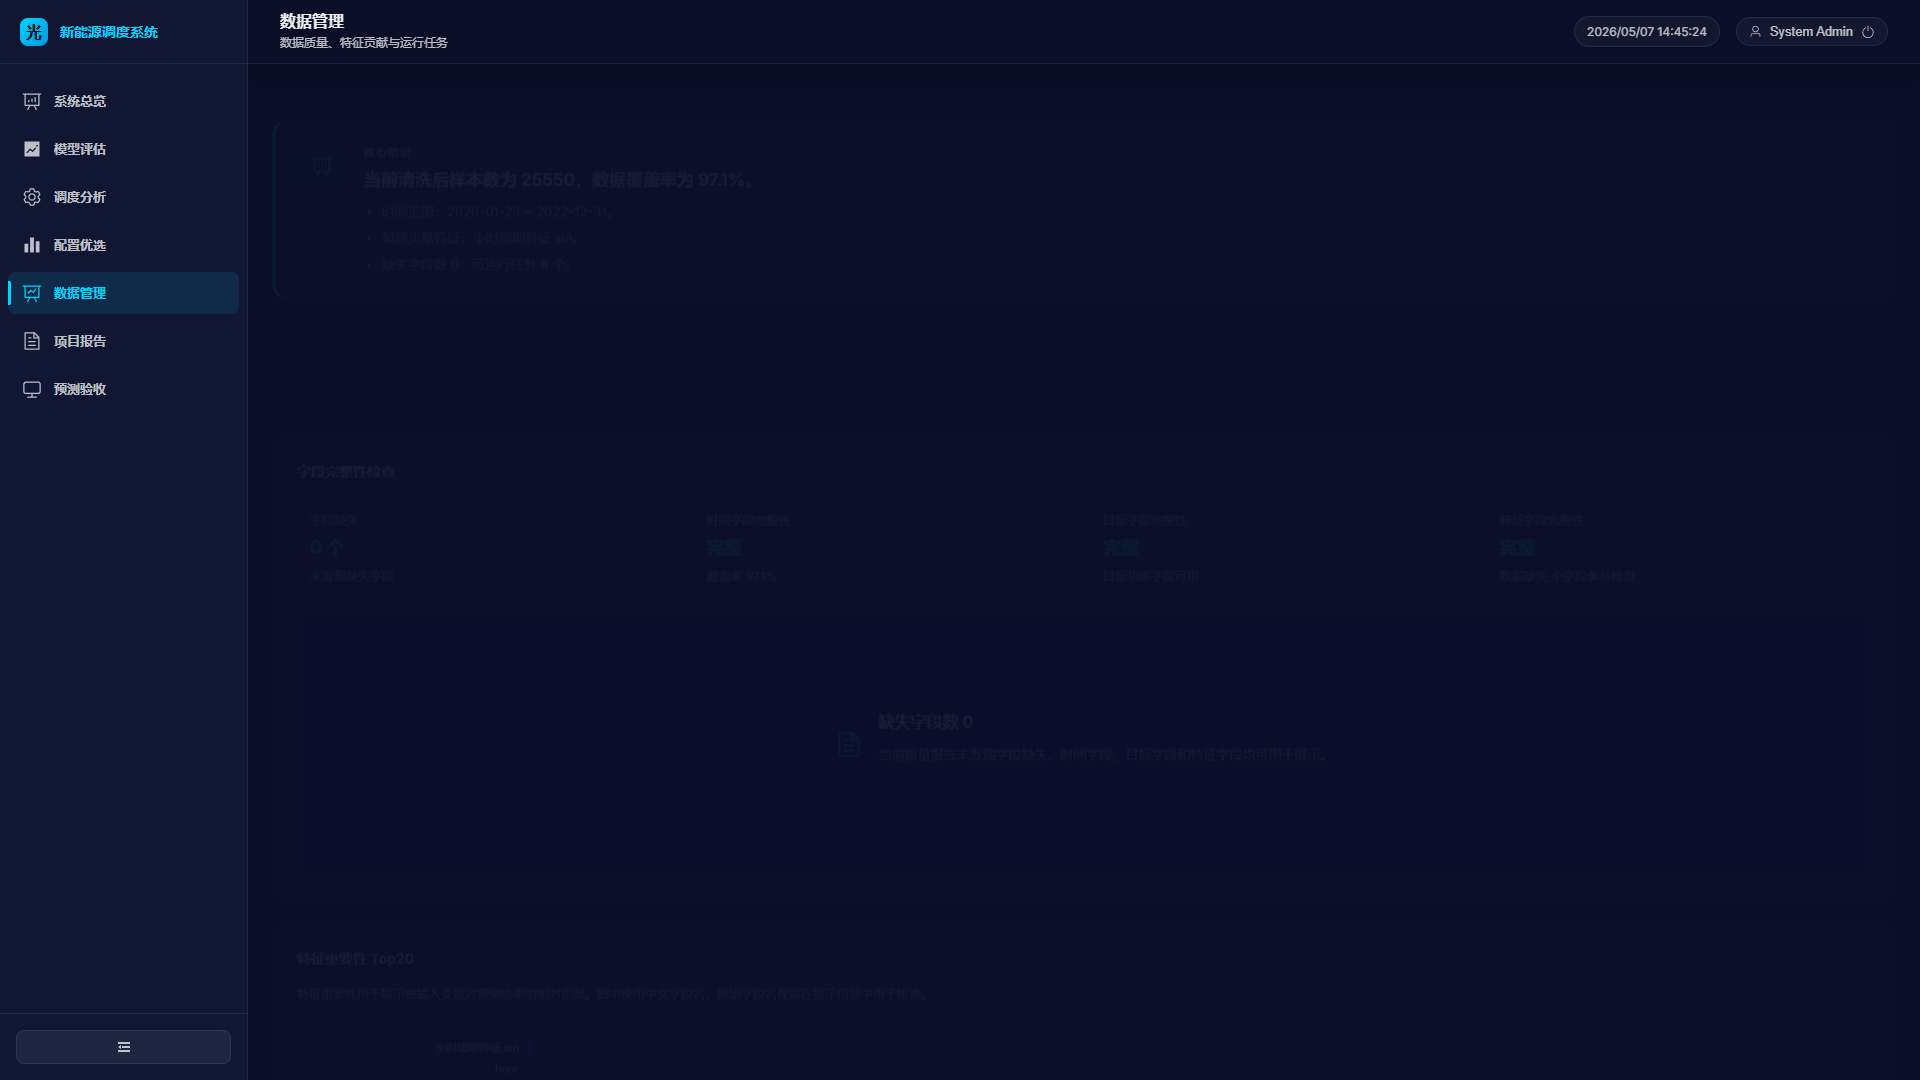
\includegraphics[width=0.92\textwidth]{figures/frontend/frontend_reports.png}
  \caption{项目报告浏览界面}
  \label{fig:frontend-reports}
\end{figure}

\section{实验分析与对比}

\subsection{光伏预测模型对比}

表\ref{tab:model-comparison}汇总了主要预测模型在$t+24h$目标上的测试集性能。所有模型使用相同的时间切分和特征集（\texttt{history\_only}，不含未来天气信息），确保对比的公平性。

\begin{table}[H]
\centering
\caption{光伏预测模型性能对比（测试集，$t+24h$）}
\label{tab:model-comparison}
\begin{tabular}{@{}lcccc@{}}
\toprule
\textbf{模型} & \textbf{nRMSE} & \textbf{日间nRMSE} & \textbf{RMSE (kW)} & \textbf{MAE (kW)} \\
\midrule
Persistence（基线）   & 0.1520 & 0.2237 & 0.1702 & 0.0901 \\
LightGBM（tuned）     & \textbf{0.1225} & \textbf{0.1689} & \textbf{0.1372} & \textbf{0.0739} \\
XGBoost              & 0.1272 & 0.1745 & 0.1425 & 0.0778 \\
CatBoost             & 0.1238 & 0.1701 & 0.1387 & 0.0751 \\
RandomForest         & 0.1237 & 0.1703 & 0.1386 & 0.0749 \\
TCN（168h窗口）       & 0.1159 & 0.1599 & 0.1298 & 0.0702 \\
CNN-LSTM（96h窗口）   & 0.1232 & 0.1686 & 0.1380 & 0.0740 \\
Attention-LSTM（96h） & 0.1512 & 0.1991 & 0.1693 & 0.0904 \\
\bottomrule
\end{tabular}
\end{table}

从表中可以得出以下分析结论：

（1）所有机器学习/深度学习模型均优于Persistence基线（nRMSE=0.1520），证明了模型确实学到了超出"用当前值预测未来"的有用信息。\cite{pv-deep-review-2025}

（2）在\texttt{history\_only}安全特征组下，LightGBM（nRMSE=0.1225）仍是综合最优模型。TCN（0.1159）在nRMSE上略优于LightGBM（改善0.0066），但TCN使用168小时长窗口和更复杂的架构，工程部署和维护成本显著高于LightGBM。CNN-LSTM（0.1232）与LightGBM基本持平。\cite{lightgbm-2017,tcn-wan-2019,wang-cnn-lstm-2019}

（3）深度学习模型（TCN、CNN-LSTM）在\texttt{weather\_history\_target\_aligned}特征组（包含历史太阳资源信息）下取得了更好的nRMSE（0.1137--0.1138），但该特征组在真实预报场景下不可用，只能作为方法验证的离线上限。\cite{pv-deep-review-2025,tcn-wan-2019,wang-cnn-lstm-2019}

（4）Attention-LSTM在\texttt{history\_only}特征组下表现最弱（nRMSE=0.1512），注意力机制在中小规模数据集上的训练稳定性不足，不建议继续围绕Attention-LSTM做无边界调参。

\subsection{储能调度策略对比}

表\ref{tab:dispatch-comparison}汇总了各调度策略在相同预测输入和电价条件下的收益对比。

\begin{table}[H]
\centering
\caption{储能调度策略收益对比（2020--2022，OPSD映射电价）}
\label{tab:dispatch-comparison}
\begin{tabular}{@{}lcccc@{}}
\toprule
\textbf{策略} & \textbf{总收益(EUR)} & \textbf{增量收益(EUR)} & \textbf{放电量(kWh)} & \textbf{等效循环} \\
\midrule
无储能（baseline）        & 136.4921 & 0.0000  & —      & — \\
固定阈值（Stage10）       & 136.4694 & -0.0227 & 0.00   & 0.00 \\
分位数阈值（Stage11最优） & 139.1494 & 2.6573  & 250.83 & 111.98 \\
滚动优化（Stage12）       & 137.1022 & 0.6100  & 378.45 & 168.95 \\
配置优化Pareto（Stage15） & 138.3900 & 1.8979  & —      & 99.99 \\
\bottomrule
\end{tabular}
\end{table}

分析要点：

（1）Stage10固定阈值策略的放电阈值为45 EUR/MWh，而当前OPSD映射电价最大值为37.67 EUR/MWh，导致整个仿真周期无放电动作。该结果表明固定阈值策略的先决条件是阈值参数与电价分布匹配，也说明了后续敏感性分析和自适应策略的必要性。

（2）Stage11分位数阈值扫描发现了最佳策略q40\_q95（充电阈值24.58、放电阈值35.70 EUR/MWh），相对无储能基线增量收益2.6573 EUR。该策略是离线全数据回看结果，不能直接固化为生产策略（优化过程已看到全部电价数据），但为后续滚动策略提供了可行的参数区间参考。

（3）Stage12滚动优化增量收益0.6100 EUR，正收益但低于Stage11离线最优。原因是滚动策略引入了循环成本、短缺惩罚和SOC终端约束，这些保守项使得策略不追求极端的充放电操作，更贴近工程实际。

（4）Stage15最优Pareto配置（cap1p5\_pow0p5\_obj3：容量3.36 kWh、功率0.28 kW）增量收益1.8979 EUR。该结果说明通过调整储能配置和目标函数惩罚项，可以在滚动优化框架内显著提升收益，比继续调整预测模型更有价值。

\subsection{策略蒸馏性能}

Stage20B两阶段神经网络策略蒸馏在测试集上取得了优异的性能指标，如表\ref{tab:distillation-results}所示。

\begin{table}[H]
\centering
\caption{两阶段策略蒸馏测试集性能}
\label{tab:distillation-results}
\begin{tabular}{@{}lc@{}}
\toprule
\textbf{指标} & \textbf{数值} \\
\midrule
动作类型准确率（Stage 1三分类） & 0.9908 \\
宏平均F1分数 & 0.9749 \\
放电召回率（discharge recall） & 0.9804 \\
充电→放电误分类数 & 0 \\
放电→充电误分类数 & 0 \\
\bottomrule
\end{tabular}
\end{table}

关键结论：放电→充电和充电→放电的误分类数均为0，说明策略蒸馏的最严重错误（将放电误判为充电，或将充电误判为放电）被完全杜绝。这一结果得益于两阶段设计——第一阶段先做粗粒度的动作类型分类，第二阶段再做精细化的功率选择——使得模型在安全关键（safety-critical）的动作类型判断上达到了极高的精度。

\subsection{Rawhide真实电站参照仿真}

表\ref{tab:rawhide-results}汇总了Rawhide Prairie Solar电站参照仿真（22 MW\_AC PV + 1 MW/2 MWh BESS）的主要结果。

\begin{table}[H]
\centering
\caption{Rawhide参照仿真结果汇总}
\label{tab:rawhide-results}
\begin{tabular}{@{}lc@{}}
\toprule
\textbf{指标} & \textbf{数值} \\
\midrule
PV容量缩放因子 & 19642.857 \\
滚动优化增量收益（相对无储能） & 1742.82 EUR \\
Stage11离线阈值上界 & 3178.40 EUR \\
Stage10固定阈值增量 & -18.86 EUR \\
推荐Pareto配置 & cap1p5\_pow1p5\_obj1 \\
Pareto配置增量收益 & 2695.23 EUR \\
退化后SOH & 0.9276 \\
退化后净增量 & -19990.48 EUR \\
\bottomrule
\end{tabular}
\end{table}

需要强调的是，Rawhide仿真中的PV出力是对PVDAQ System 10数据按容量比例缩放得到的，不是Rawhide电站的实测小时级发电数据；电价仍使用OPSD映射电价，不是Colorado/Platte River真实市场结算价格。因此，所有收益数据应理解为"在真实电站容量参数和项目代理电价下的调度可行性评估"，不能表述为"Rawhide历史运行收益复盘"。

\subsection{天气驱动与价格场景仿真}

Stage21实现了Rawhide坐标下的Open-Meteo天气驱动PV出力估算和5类可配置电价场景的调度仿真：

\begin{table}[H]
\centering
\caption{Stage21五类价格场景滚动优化增量收益}
\label{tab:stage21}
\begin{tabular}{@{}lcc@{}}
\toprule
\textbf{价格场景} & \textbf{增量收益(EUR)} & \textbf{电价特征} \\
\midrule
flat\_proxy\_30        & 0.0000   & 恒定30 EUR/MWh，无套利空间 \\
tou\_peak\_valley       & 104.8543 & 峰谷分时电价 \\
solar\_duck\_curve       & 217.2114 & 午间低谷、晚间高峰（鸭子曲线） \\
high\_volatility\_stress & 601.6364 & 高波动压力测试 \\
opsd\_profile\_reference & 35.4851  & OPSD映射电价分布参考 \\
\bottomrule
\end{tabular}
\end{table}

该结果证明了以下两点：（1）在Rawhide坐标下的天气驱动PV出力估算和价格场景配置方案是可实现的；（2）收益对电价场景的敏感性极高——在鸭子曲线和高波动场景下收益显著提升，在恒定电价下无套利空间。但该收益基于合成电价场景和物理估算PV出力，不能外推为Rawhide真实市场结算收益。

\section{性能测试}

\subsection{后端性能}

\begin{table}[H]
\centering
\caption{后端关键操作性能}
\label{tab:perf-backend}
\begin{tabular}{@{}lccc@{}}
\toprule
\textbf{操作} & \textbf{数据规模} & \textbf{耗时} & \textbf{评价} \\
\midrule
LightGBM训练 & 7万样本, 50+特征 & $<$10s & 优秀 \\
全年调度仿真（固定阈值） & 25255个交付时刻 & $<$5s & 优秀 \\
全年滚动优化调度 & 25255个交付时刻 & $\sim$30s & 可接受 \\
Stage15 27组配置扫描 & 25255×27交付时刻 & $\sim$3min & 可接受 \\
深度学习训练（CNN-LSTM, 100epoch） & 7万样本 & $\sim$10min & 可接受 \\
API GET响应（$\le$1000行） & — & $<$200ms & 满足要求 \\
\bottomrule
\end{tabular}
\end{table}

\subsection{前端性能}

前端经过Vite manual chunks优化后的构建产物如表\ref{tab:perf-frontend}所示。

\begin{table}[H]
\centering
\caption{前端构建产物拆分}
\label{tab:perf-frontend}
\begin{tabular}{@{}lcc@{}}
\toprule
\textbf{Chunk} & \textbf{大小(kB)} & \textbf{说明} \\
\midrule
main entry & 9.48 & 应用入口，路由和状态 \\
vue-vendor & 24.85 & Vue 3运行时 \\
markdown & 63.70 & Markdown渲染库 \\
charts & 697.56 & ECharts + vue-echarts \\
element-plus & 889.56 & Element Plus UI组件库 \\
\bottomrule
\end{tabular}
\end{table}

主入口JS从优化前的约1389 kB降至优化后的9.48 kB，首屏加载时间显著缩短。Element Plus和ECharts作为最大chunk，后续可通过按需导入进一步拆分。

\section{测试结论与改进方向}

综合功能测试、实验分析和性能测试结果，系统各模块均通过质量门禁验证，主要指标满足非功能需求。当前系统存在以下已知局限和可改进方向：

\begin{enumerate}[label=(\arabic*)]
  \item \textbf{电价数据局限}：OPSD映射电价仅为德国电力市场画像，不是Colorado/PSCO同区域真实小时级结算价格。基于此电价的收益结论只能作为离线敏感性分析，不能作为真实商业收益预测。\cite{opsd-datapackage-2020,opsd-wiese-2019}
  \item \textbf{光伏预测天花板}：LightGBM nRMSE=0.1225是当前数据集上的最佳性能。考虑到光伏出力的固有随机性（云层遮挡等），继续在单一数据集上调参的边际收益递减。未来改进方向应聚焦于引入更高分辨率的天气预报数据（如HRRR 3km网格数据）和多数据源的ensemble预测。\cite{lightgbm-2017}
  \item \textbf{策略蒸馏的泛化性}：Stage20B两阶段策略蒸馏在离线回放测试集上达到了0.9908的准确率，但其在真实实时调度场景下的泛化性（尤其是面对price regime change时的表现）尚需在线验证。\cite{policy-distillation-2016}
  \item \textbf{电池退化模型的简化}：当前退化模型基于文献查表的简化SOH-循环深度关系，未考虑温度、充放电倍率（C-rate）和日历老化等因素。未来可引入更精细的电化学退化模型或数据驱动退化预测。\cite{battery-degradation-review-2021,rainflow-soc-2022}
  \item \textbf{前端包体优化}：Element Plus全量引入和ECharts全量引入导致chunk偏大，后续可考虑按需组件导入和图表库的轻量化替代方案。
\end{enumerate}

\section{本章小结}

本章从功能测试和性能测试两个维度对系统进行了全面评估。后端9个单元测试和12个API契约测试全部通过，前端6个E2E测试全部通过。实验分析部分系统对比了8个预测模型的性能差异，分析了4类调度策略的收益逻辑，验证了两阶段策略蒸馏的优异性能，呈现了Rawhide参照仿真和天气驱动场景仿真的结果。性能测试表明系统各操作耗时在可接受范围内，前端构建优化后主入口JS压缩至9.48 kB。最后指出了5个已知局限和改进方向。

% ============================================================
%  第七章 总结与展望
% ============================================================
\chapter{总结与展望}

\section{完成的工作总结}

本文设计并实现了一套完整的新能源储能调度仿真系统，主要完成了以下工作：

（1）\textbf{数据地基构建}：从PVDAQ、NSRDB、OPSD和Open-Meteo四个公开数据源采集并标准化了覆盖2020--2022年三年的小时级数据，经过数据清洗、时间对齐和特征工程，构建了包含50+特征的标准化数据集。\cite{pvdaq-nrel,nsrdb-nrel,opsd-datapackage-2020,opsd-wiese-2019,open-meteo-2023}

（2）\textbf{光伏功率预测}：以LightGBM梯度提升树为主模型，在$t+24h$预测任务上取得nRMSE=0.1225（日间0.1689）的性能。系统对比了7种表格模型和3种深度学习模型（TCN、CNN-LSTM、Attention-LSTM），完成了从模型选择、训练、推理固化到预测产物消费的完整管线。\cite{lightgbm-2017,tcn-wan-2019,wang-cnn-lstm-2019,qu-attention-cnnlstm-2021}

（3）\textbf{储能调度优化}：实现了固定阈值调度、分位数阈值敏感性分析（26组策略）、24小时前瞻滚动优化和储能配置敏感性分析（27组配置）的完整策略演进。滚动优化在保证全部物理约束的前提下取得正增量收益（0.6100 EUR），最优Pareto配置增量收益达1.8979 EUR。\cite{bess-review-2023,bo-two-stage-rolling-2025,li-mpc-microgrid-2025}

（4）\textbf{神经网络策略蒸馏}：提出两阶段策略蒸馏框架（动作类型分类 + 功率细化），以滚动优化为教师策略，学生模型在测试集上动作类型准确率0.9908，Macro-F1 0.9749，且充电-放电致命误分类数为0。\cite{policy-distillation-2016}

（5）\textbf{真实电站参照仿真}：以Rawhide Prairie Solar（22 MW\_AC PV + 1 MW/2 MWh BESS）公开参数为参照，完成容量缩放全链路仿真，验证了系统架构对真实电站参数的适配能力。\cite{rawhide-nrel}

（6）\textbf{电池退化分析}：基于雨流计数法实现了SOC循环识别和SOH退化模拟，评估了电池老化对调度净收益的长期影响。\cite{battery-degradation-review-2021,rainflow-soc-2022}

（7）\textbf{可视化展示平台}：基于Vue 3 + FastAPI实现了前后端分离的Web可视化系统，涵盖6个功能页面，并通过JWT认证、DOMPurify XSS防护、CORS白名单和响应式布局完成生产化安全加固。\cite{vue3,fastapi,jwt-rfc7519,dompurify,owasp-top10-2021}

（8）\textbf{天气驱动扩展验证}：接入Open-Meteo天气API和可配置电价场景（5类），实现了Rawhide坐标下天气驱动光伏估算和多场景调度仿真。\cite{open-meteo-2023,rawhide-nrel}

\section{系统的核心贡献}

本系统的核心贡献不在于单一算法的突破，而在于构建了一条从数据到决策的\textbf{完整可复现实验链路}，并在此链路上完成了多阶段、多策略、多场景的系统性验证。具体而言：

\textbf{工程贡献}：建立了一套门禁驱动的质量保证体系——每个Stage的实验输出在进入下游消费前必须通过SOC、功率、时间泄漏、特征完整性等多维硬性门禁，确保全链路的物理可行性和数据完整性。

\textbf{方法贡献}：提出了两阶段神经网络策略蒸馏方法，将复杂优化策略（24小时前瞻滚动优化）压缩为学生神经网络模型，在保证高精度的同时将推理计算复杂度从$O(H^2)$降至$O(1)$。\cite{policy-distillation-2016,bo-two-stage-rolling-2025,li-mpc-microgrid-2025}

\textbf{方法论贡献}：验证了"传统机器学习预测 + 滚动优化调度 + 神经网络策略蒸馏"这一混合技术路线的可行性——在预测侧接受传统模型的稳健性，在调度侧拥抱深度学习的决策效率。\cite{lightgbm-2017,bo-two-stage-rolling-2025,li-mpc-microgrid-2025,policy-distillation-2016}

\section{系统不足与未来改进方向}

（1）\textbf{预测精度提升}：当前预测模型基于NSRDB历史太阳资源数据，在真实预报场景下的精度可能下降。未来可引入HRRR高分辨率数值天气预报的完整cycle/lead-time信息，提高真实预报场景下的预测精度。\cite{nsrdb-nrel}

（2）\textbf{真实市场结算}：当前收益计算基于OPSD德国电价画像，不是Colorado/PSCO同区域真实市场结算价格。未来可接入2023年4月后SPP WEIS RTBM LMP数据作为扩展验证（但不替换主实验期结算口径）。\cite{opsd-datapackage-2020,opsd-wiese-2019}

（3）\textbf{策略蒸馏泛化}：两阶段策略蒸馏在离线回放测试集上表现优异，但未在真实实时调度或price regime change场景下验证。未来可进行在线RL微调或domain randomization增强泛化性。\cite{policy-distillation-2016}

（4）\textbf{电池退化模型增强}：当前退化模型基于简化查表法，未来可引入电化学模型（如单粒子模型SPM）或数据驱动SOH估计（如基于电压-容量曲线的特征提取）。\cite{battery-degradation-review-2021}

（5）\textbf{多站联合调度}：当前系统为单站单储能调度，未来可扩展至多电站、多储能单元的协同优化调度。\cite{cn-storage-config-review-2025,bo-two-stage-rolling-2025,li-mpc-microgrid-2025}

（6）\textbf{前端工程化}：当前Element Plus和ECharts全量引入导致chunk偏大，未来可实施按需组件导入和路由级异步加载进一步优化首屏性能。

\section{本章小结}

本章总结了系统完成的八项核心工作，提炼了工程贡献（门禁驱动质量保证）、方法贡献（两阶段策略蒸馏）和方法论贡献（混合技术路线验证）三个层面的核心价值，并指出了六个未来的改进方向。总体而言，系统已形成一个从数据采集到可视化展示的完整闭环，具备工程演示和学术论文的双重价值。

% ============================================================
%  参考文献
% ============================================================
\begin{thebibliography}{99}

\bibitem{iea-pvps-2025}
International Energy Agency Photovoltaic Power Systems Programme. Snapshot of Global PV Markets 2025[R]. Paris: IEA PVPS, 2025.

\bibitem{duck-curve-caiso-2016}
California Independent System Operator. What the Duck Curve Tells Us About Managing a Green Grid[R/OL]. 2016.

\bibitem{bess-review-2023}
Hesse H C, Schimpe M, Kucevic D, Jossen A. Lithium-ion battery storage for the grid: A review of stationary battery storage system design tailored for applications in modern power grids[J]. Energies, 2017,10(12):2107. DOI:10.3390/en10122107.
\bibitem{cn-storage-config-review-2025}
葛磊蛟，郑轶文，李小平，等. 高比例分布式光伏接入下配电网多类型储能优化配置技术综述[J]. 浙江电力，2025，44(5)：1--11.

\bibitem{xie-hybrid-storage-2021}
谢丽蓉，郑浩，魏成伟，等. 兼顾补偿预测误差和平抑波动的光伏混合储能协调控制策略[J]. 电力系统自动化，2021，45(3)：130--138.

\bibitem{pv-physical-model-2019}
Dolara A, Leva S, Manzolini G. Comparison of different physical models for PV power output prediction[J]. Solar Energy, 2015,119:83--99. DOI:10.1016/j.solener.2015.06.017.
\bibitem{lightgbm-2017}
Ke G, Meng Q, Finley T, et al. LightGBM: A highly efficient gradient boosting decision tree[C]//Advances in Neural Information Processing Systems 30. 2017:3149--3157.

\bibitem{pv-deep-review-2025}
张沛，曹泽凯，付学谦，等. 基于深度学习的光伏功率预测方法研究综述[J]. 电力信息与通信技术，2025，23(12)：78--88.

\bibitem{lstm-pv-2021}
Qing X, Niu Y. Hourly day-ahead solar irradiance prediction using weather forecasts by LSTM[J]. Energy, 2021,222:119932. DOI:10.1016/j.energy.2021.119932.
\bibitem{tcn-wan-2019}
Bai S, Kolter J Z, Koltun V. An empirical evaluation of generic convolutional and recurrent networks for sequence modeling[EB/OL]. arXiv:1803.01271, 2018.

\bibitem{wang-cnn-lstm-2019}
Wang K, Qi X, Liu H. Photovoltaic power forecasting based LSTM-convolutional network[J]. Energy, 2019,189:116225.

\bibitem{qu-attention-cnnlstm-2021}
Qu J, Qian Z, Pei Y. Day-ahead hourly photovoltaic power forecasting using attention-based CNN-LSTM neural network embedded with multiple relevant and target variables prediction pattern[J]. Energy, 2021,232:120996.

\bibitem{milp-dispatch-2021}
Padmanabhan N, Ahmed M, Bhattacharya K. Battery energy storage systems in energy and reserve markets[J]. IEEE Transactions on Power Systems, 2021,36(1):440--453.

\bibitem{bo-two-stage-rolling-2025}
薄利明，邹鹏，郑惠萍，等. 考虑源荷储联合调峰的日前-日内两阶段滚动优化调度[J]. 华北电力大学学报（自然科学版），2025(1)：34--43.

\bibitem{li-mpc-microgrid-2025}
Li D, Ren L, Liu F, et al. Two-time scale microgrid scheduling based on power fluctuation mitigation priority and model predictive control[J]. Energy, 2025,324:135760.

\bibitem{drl-energy-storage-2023}
Cao J, Harrold D, Fan Z, Morstyn T, Healey D, Li K. Deep reinforcement learning-based energy storage arbitrage with accurate lithium-ion battery degradation model[J]. IEEE Transactions on Smart Grid, 2020,11(5):4513--4521. DOI:10.1109/TSG.2020.2986333.
\bibitem{policy-distillation-2016}
Rusu A A, Colmenarejo S G, Gulcehre C, et al. Policy distillation[C]//International Conference on Learning Representations. 2016.

\bibitem{battery-degradation-review-2021}
Edge J S, O'Kane S, Prosser J, et al. Lithium ion battery degradation: What you need to know[J]. Physical Chemistry Chemical Physics, 2021,23(14):8200--8221.

\bibitem{rainflow-soc-2022}
Downing S D, Socie D F. Simple rainflow counting algorithms[J]. International Journal of Fatigue, 1982,4(1):31--40.
\bibitem{open-meteo-2023}
Zippenfenig P. Open-Meteo.com Weather API[DS/OL]. Zenodo, 2023. DOI:10.5281/zenodo.7970649.

\bibitem{pvdaq-nrel}
Deline C, Perry K, Deceglie M, et al. Photovoltaic Data Acquisition (PVDAQ) Public Datasets[DS/OL]. Golden: National Renewable Energy Laboratory, 2021. DOI:10.25984/1846021.

\bibitem{nsrdb-nrel}
Sengupta M, Xie Y, Lopez A, et al. The National Solar Radiation Database (NSRDB)[J]. Renewable and Sustainable Energy Reviews, 2018,89:51--60.

\bibitem{opsd-datapackage-2020}
Open Power System Data. Time series data package[DS/OL]. 2020. \url{https://data.open-power-system-data.org/time_series/}.

\bibitem{opsd-wiese-2019}
Wiese F, Schlecht I, Bunke W D, et al. Open Power System Data: Frictionless data for electricity system modelling[J]. Applied Energy, 2019,236:401--409.

\bibitem{rawhide-nrel}
Platte River Power Authority. New solar project operational: Rawhide Prairie Solar to produce 22 MW solar, 2 MWh battery storage[EB/OL]. 2021. \url{https://prpa.org/news-releases/new-solar-project-operational/}.
\bibitem{fastapi}
FastAPI. FastAPI documentation[EB/OL]. 2026. \url{https://fastapi.tiangolo.com/}.
\bibitem{vue3}
Vue.js Core Team. Vue.js documentation[EB/OL]. 2026. \url{https://vuejs.org/}.
\bibitem{xgboost-2016}
Chen T, Guestrin C. XGBoost: A scalable tree boosting system[C]//Proceedings of the 22nd ACM SIGKDD International Conference on Knowledge Discovery and Data Mining. 2016:785--794.

\bibitem{catboost-2018}
Prokhorenkova L, Gusev G, Vorobev A, et al. CatBoost: unbiased boosting with categorical features[C]//Advances in Neural Information Processing Systems 31. 2018:6638--6648.

\bibitem{random-forest-2001}
Breiman L. Random forests[J]. Machine Learning, 2001,45(1):5--32.

\bibitem{scikit-learn-2011}
Pedregosa F, Varoquaux G, Gramfort A, et al. Scikit-learn: Machine learning in Python[J]. Journal of Machine Learning Research, 2011,12:2825--2830.

\bibitem{pytorch-2019}
Paszke A, Gross S, Massa F, et al. PyTorch: An imperative style, high-performance deep learning library[C]//Advances in Neural Information Processing Systems 32. 2019:8024--8035.

\bibitem{design-patterns}
Gamma E, Helm R, Johnson R, Vlissides J. Design Patterns: Elements of Reusable Object-Oriented Software[M]. Boston: Addison-Wesley, 1994.

\bibitem{jwt-rfc7519}
Jones M, Bradley J, Sakimura N. JSON Web Token (JWT)[S/OL]. RFC 7519, 2015. \url{https://www.rfc-editor.org/rfc/rfc7519}.

\bibitem{owasp-top10-2021}
OWASP Foundation. OWASP Top 10:2021[EB/OL]. 2021. \url{https://owasp.org/Top10/}.

\bibitem{dompurify}
Cure53. DOMPurify Documentation[EB/OL]. 2024. \url{https://github.com/cure53/DOMPurify}.

\end{thebibliography}

% ============================================================
%  附录
% ============================================================
\appendix
\chapter{核心代码片段}

\section{数据标准化核心函数}

\begin{lstlisting}[caption={多源数据时间标准化}, label={lst:appendix-1}]
def standardize_multi_source_data(
    pvdaq_df: pd.DataFrame,
    nsrdb_df: pd.DataFrame,
    opsd_df: pd.DataFrame
) -> pd.DataFrame:
    """将三个数据源合并为统一的标准化 DataFrame."""
    # PVDAQ: MST/MDT -> UTC
    pvdaq_df['ts'] = pd.to_datetime(pvdaq_df['ts_local'])
    pvdaq_df['ts'] = pvdaq_df['ts'].dt.tz_localize(
        'America/Denver', ambiguous='infer'
    ).dt.tz_convert('UTC').dt.floor('h')

    # NSRDB: already UTC
    nsrdb_df['ts'] = pd.to_datetime(nsrdb_df['time_utc']).dt.floor('h')

    # OPSD: CET/CEST -> UTC
    opsd_df['ts'] = pd.to_datetime(opsd_df['utc_timestamp']).dt.floor('h')

    # Merge on common UTC hour
    merged = pvdaq_df.merge(nsrdb_df, on='ts', how='inner')
    merged = merged.merge(opsd_df, on='ts', how='left')

    return merged.sort_values('ts')
\end{lstlisting}

\section{物理约束审计函数}

\begin{lstlisting}[caption={调度物理约束审计}, label={lst:appendix-2}]
def audit_dispatch_constraints(results: pd.DataFrame,
                               capacity_kwh: float,
                               max_power_kw: float) -> dict:
    """SOC、功率、同时充放电和能量守恒审计."""
    gates = {}

    # SOC bounds
    gates['soc_within_bounds'] = (
        (results['soc_kwh'] >= 0.1 * capacity_kwh).all() and
        (results['soc_kwh'] <= 0.9 * capacity_kwh).all()
    )

    # Power bounds
    gates['charge_power_within_bounds'] = (
        results['charge_kw'].between(0, max_power_kw).all()
    )
    gates['discharge_power_within_bounds'] = (
        results['discharge_kw'].between(0, max_power_kw).all()
    )

    # No simultaneous charge/discharge
    gates['no_simultaneous_charge_discharge'] = (
        (results['charge_kw'] * results['discharge_kw'] == 0).all()
    )

    # Energy conservation
    delta_soc = results['soc_kwh'].diff().fillna(0)
    net_flow = (results['charge_kw'] * 0.90 -
                results['discharge_kw'] / 0.90)
    max_error = (delta_soc - net_flow).abs().max()
    gates['energy_conservation'] = max_error < 1e-9

    return gates
\end{lstlisting}

\chapter{前端用户界面截图附录}

本附录补充展示正文未展开的调度页页签和移动端适配截图，用于说明系统在不同分析场景和不同视口下的界面完整性。

Rawhide参考电站收益界面如图\ref{fig:appendix-rawhide}所示。该页签仍由\texttt{DispatchSimulation.vue}承载，展示Rawhide公开参数参考仿真的收益、配置和运行结果；论文中使用该图时必须保留“参考仿真、非真实结算”的边界。

\begin{figure}[H]
  \centering
  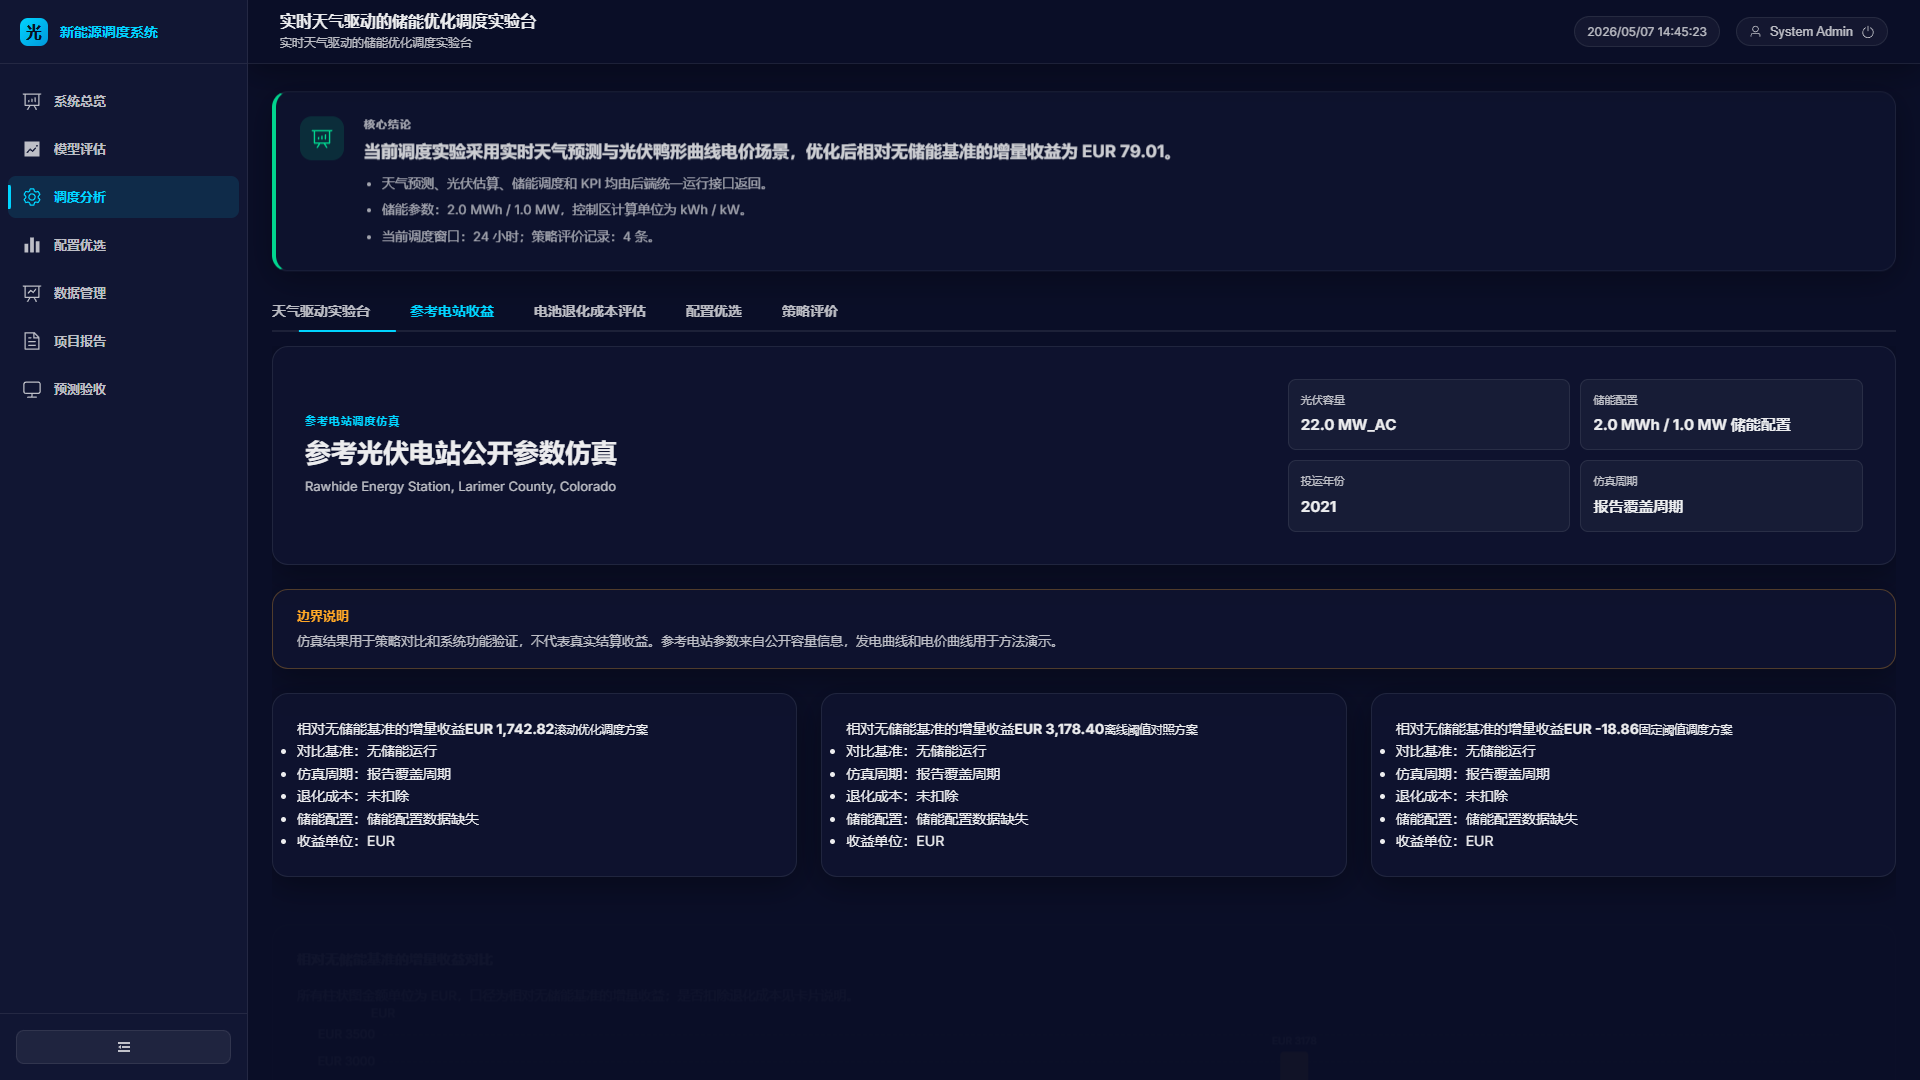
\includegraphics[width=0.92\textwidth]{figures/frontend/frontend_dispatch_rawhide.png}
  \caption{Rawhide参考电站收益界面}
  \label{fig:appendix-rawhide}
\end{figure}

电池退化成本评估界面如图\ref{fig:appendix-degradation}所示。该页签用于展示退化回放和SOH估算结果，帮助用户理解储能调度收益在纳入循环寿命成本后的变化。

\begin{figure}[H]
  \centering
  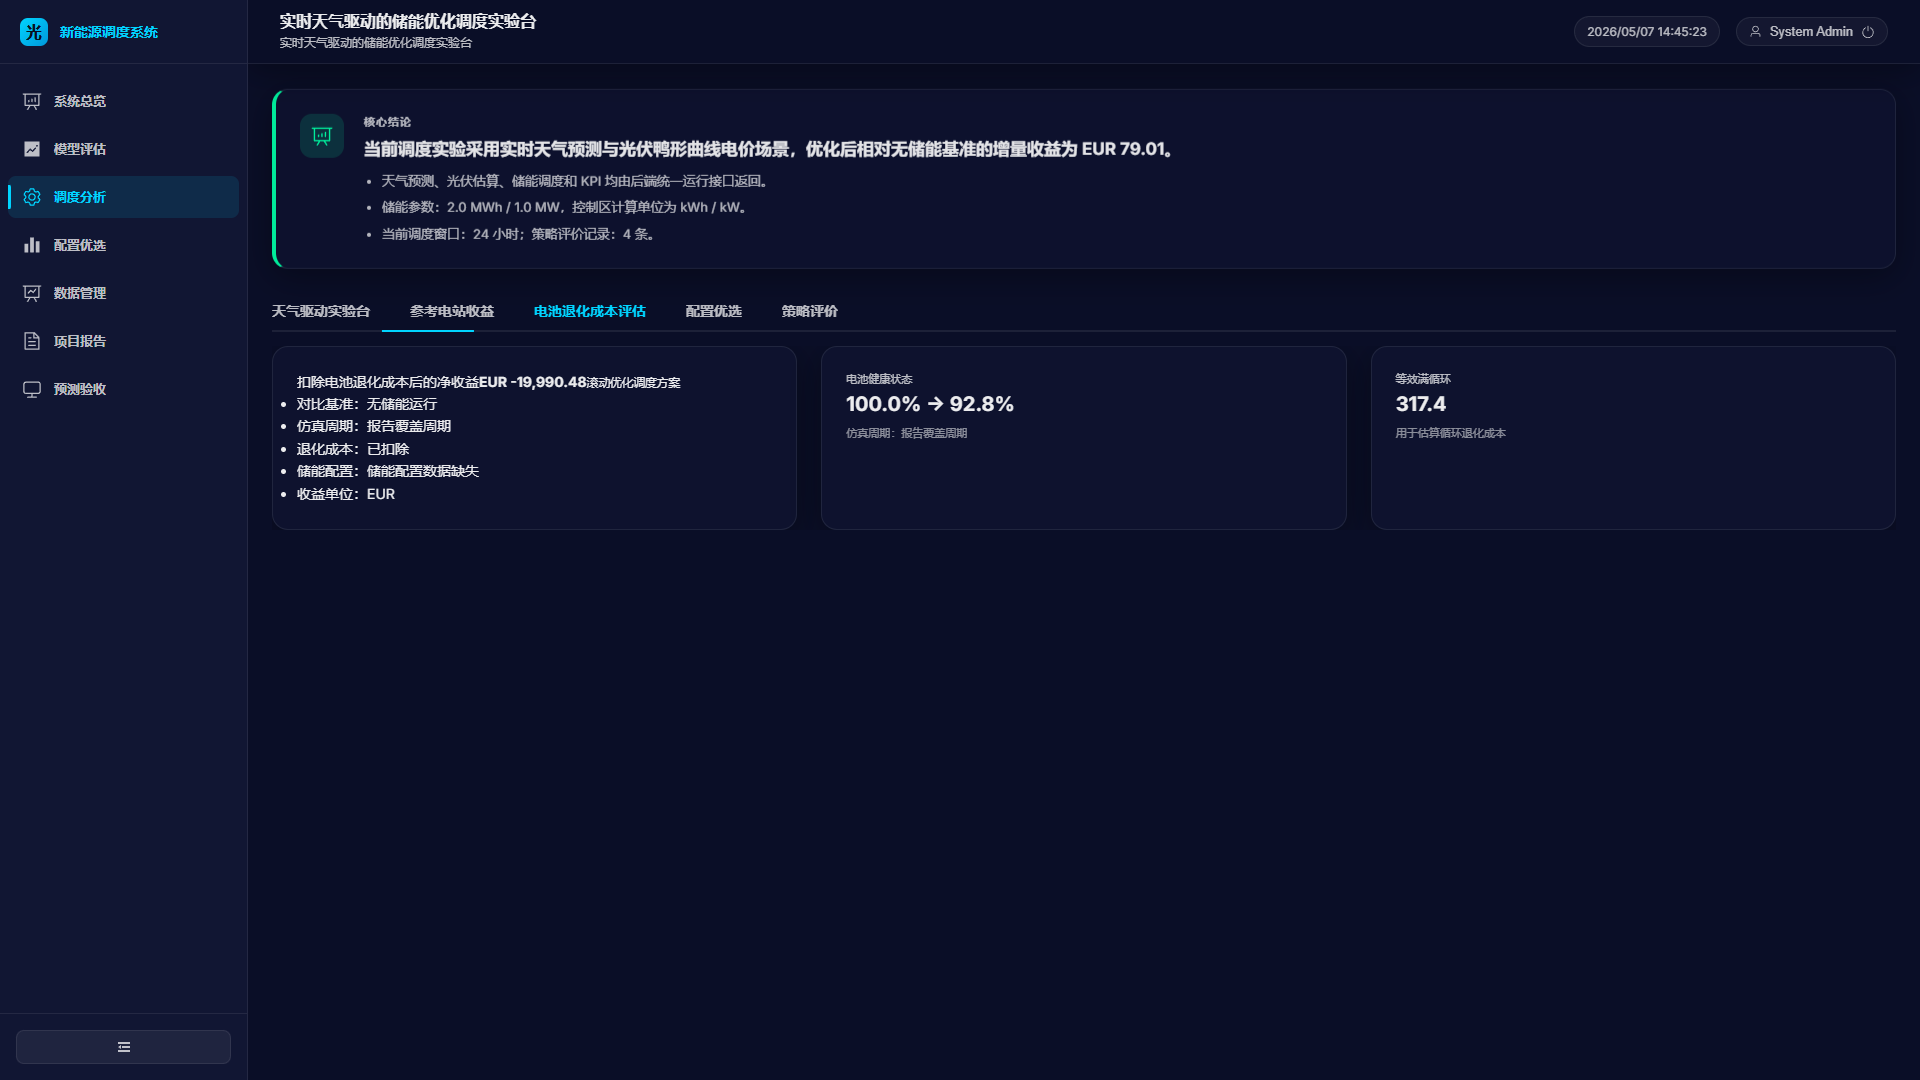
\includegraphics[width=0.92\textwidth]{figures/frontend/frontend_dispatch_degradation.png}
  \caption{电池退化成本评估界面}
  \label{fig:appendix-degradation}
\end{figure}

移动端系统总览界面如图\ref{fig:appendix-mobile-overview}所示。系统在窄屏视口下会保持导航、指标卡和图表区域的可访问性，避免横向溢出影响基本浏览。

\begin{figure}[H]
  \centering
  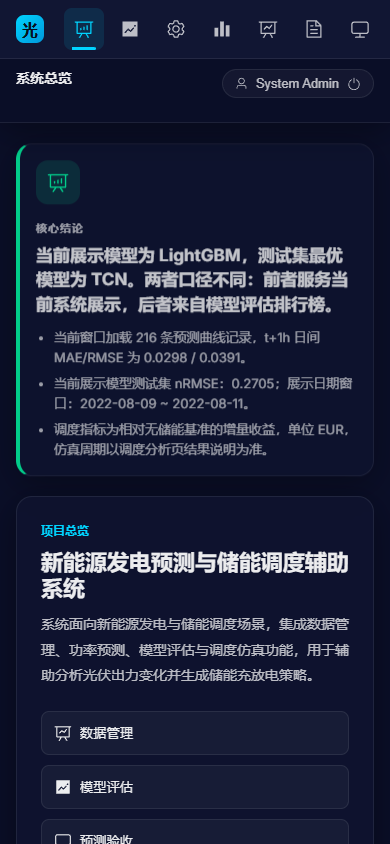
\includegraphics[width=0.45\textwidth]{figures/frontend/frontend_mobile_overview.png}
  \caption{移动端系统总览界面}
  \label{fig:appendix-mobile-overview}
\end{figure}

\chapter{系统部署与验收指南}

本附录简要描述启动系统开发服务器并进行验收的步骤。详细部署指南参见\texttt{docs/production\_deployment\_guide.md}。

\subsection*{后端启动}

\begin{lstlisting}[language=bash, caption={后端开发服务器启动}]
cd C:\Project\New_Energy_Sys
$env:PYTHONPATH='src;.'
python -m uvicorn backend.app.main:app --host 127.0.0.1 --port 8000
\end{lstlisting}

\subsection*{前端启动}

\begin{lstlisting}[language=bash, caption={前端开发服务器启动}]
cd C:\Project\New_Energy_Sys\frontend
npm run dev -- --host 127.0.0.1 --port 3000
\end{lstlisting}

\subsection*{验收命令清单}

\begin{lstlisting}[language=bash, caption={验收命令}]
# 后端 API 契约测试
$env:PYTHONPATH='src'
python scripts\api_smoke_frontend_contract.py

# 后端单元测试
python -m pytest tests\ -q

# 前端静态检查
cd frontend; npm run check

# 前端生产构建
cd frontend; npm run build

# 前端 E2E 测试（需要系统 Chrome/Edge）
cd frontend; npm run test:e2e -- --project=system-chromium
\end{lstlisting}

% ============================================================
%  致谢
% ============================================================
\chapter*{致谢}
\addcontentsline{toc}{chapter}{致谢}

在本论文完成之际，谨向在本科四年学习和毕业设计过程中给予我指导、帮助和鼓励的所有人表示诚挚的感谢。

首先，衷心感谢我的指导老师。从选题到方案设计，从实验推进到论文撰写，老师始终给予我耐心的指导和宝贵的建议。老师的严谨治学态度和对前沿技术的敏锐洞察，使我在整个毕设过程中受益匪浅。

感谢各位授课老师和辅导员，在四年的大学学习中为我打下了扎实的计算机科学基础，使我有能力独立完成这样一项综合性较强的工程项目。

感谢开源社区和公开数据提供方——PVDAQ（NREL）、NSRDB（NREL）、OPSD（Open Power System Data）和Open-Meteo——为本项目提供了高质量、可免费获取的光伏、气象和电力市场数据。没有这些公开数据，本系统将失去可复现性的基础。

最后，感谢我的家人和朋友。你们的理解、支持和鼓励是我坚持完成四年学业和毕业设计的最大动力。

\vspace{2cm}

\begin{flushright}
2026年5月
\end{flushright}

\end{document}
